\documentclass[a4paper,oneside,11pt]{article}
\usepackage{graphicx}
\usepackage{ tipa }
\usepackage{hyperref}
\usepackage{titling}
\usepackage{blindtext}
\usepackage{enumitem}
\usepackage{eurosym}
\usepackage{float}
\usepackage{listings}
\usepackage{tabularx}


\title{RASD}
\author{Daniele Montesi, Nicola Fossati, Francesco Sgherzi}
\date{\today}
\begin{document}
    \begin{titlingpage} 
        \begin{center}
            
\includegraphics[height=5cm]{assets/Logo_Politecnico_Milano.png}\\
            \vspace{4cm}
            \begin{huge} 
                \textbf{\thetitle} \\
            \end{huge}
            \vspace{0.3cm}
            \begin{Large}
                \textit{Software Engineering 2 Project - TrackMe} \\
            \end{Large}
        \end{center}
        \begin{large}
            \vspace{4cm}
            \textbf{Authors}
            \begin{itemize}
                \item Daniele Montesi - \textit{912980} 
                \item Nicola Fossati - \textit{915244}
                \item Francesco Sgherzi - \textit{915377}
            \end{itemize}
        \end{large}
    \end{titlingpage}
    \newpage
    \tableofcontents
    \newpage
    \section{Introduction}
    
        \subsection{Purpose}
            The main purpose of this document is to exhaustively describe the Data4Help main architecture, its parts and how they interact. There is also a chapter that covers the user interface.

The main recipients of this document are the project manager, developers and testers, but it can also be useful for further development reference and maintenance.
        \subsection{Scope}
            % To define the scope of the product we can use ``The World \& Machine'' approach by M. Jackson and P. Zave.
% We can define the real world entities that interact with the system (the World), the entities that belong to the system (the Machine) and the shared phenomena (the intersection of the two other sets).

% TODO: add image here

The \textit{The World and the Machine} approach is used in defining the scope of the project.
By defining the real world entities that interact with the system and the properties of the system itself we can determine the intersection between the two sets: the \textit{shared phenomena}.
\begin{center}
    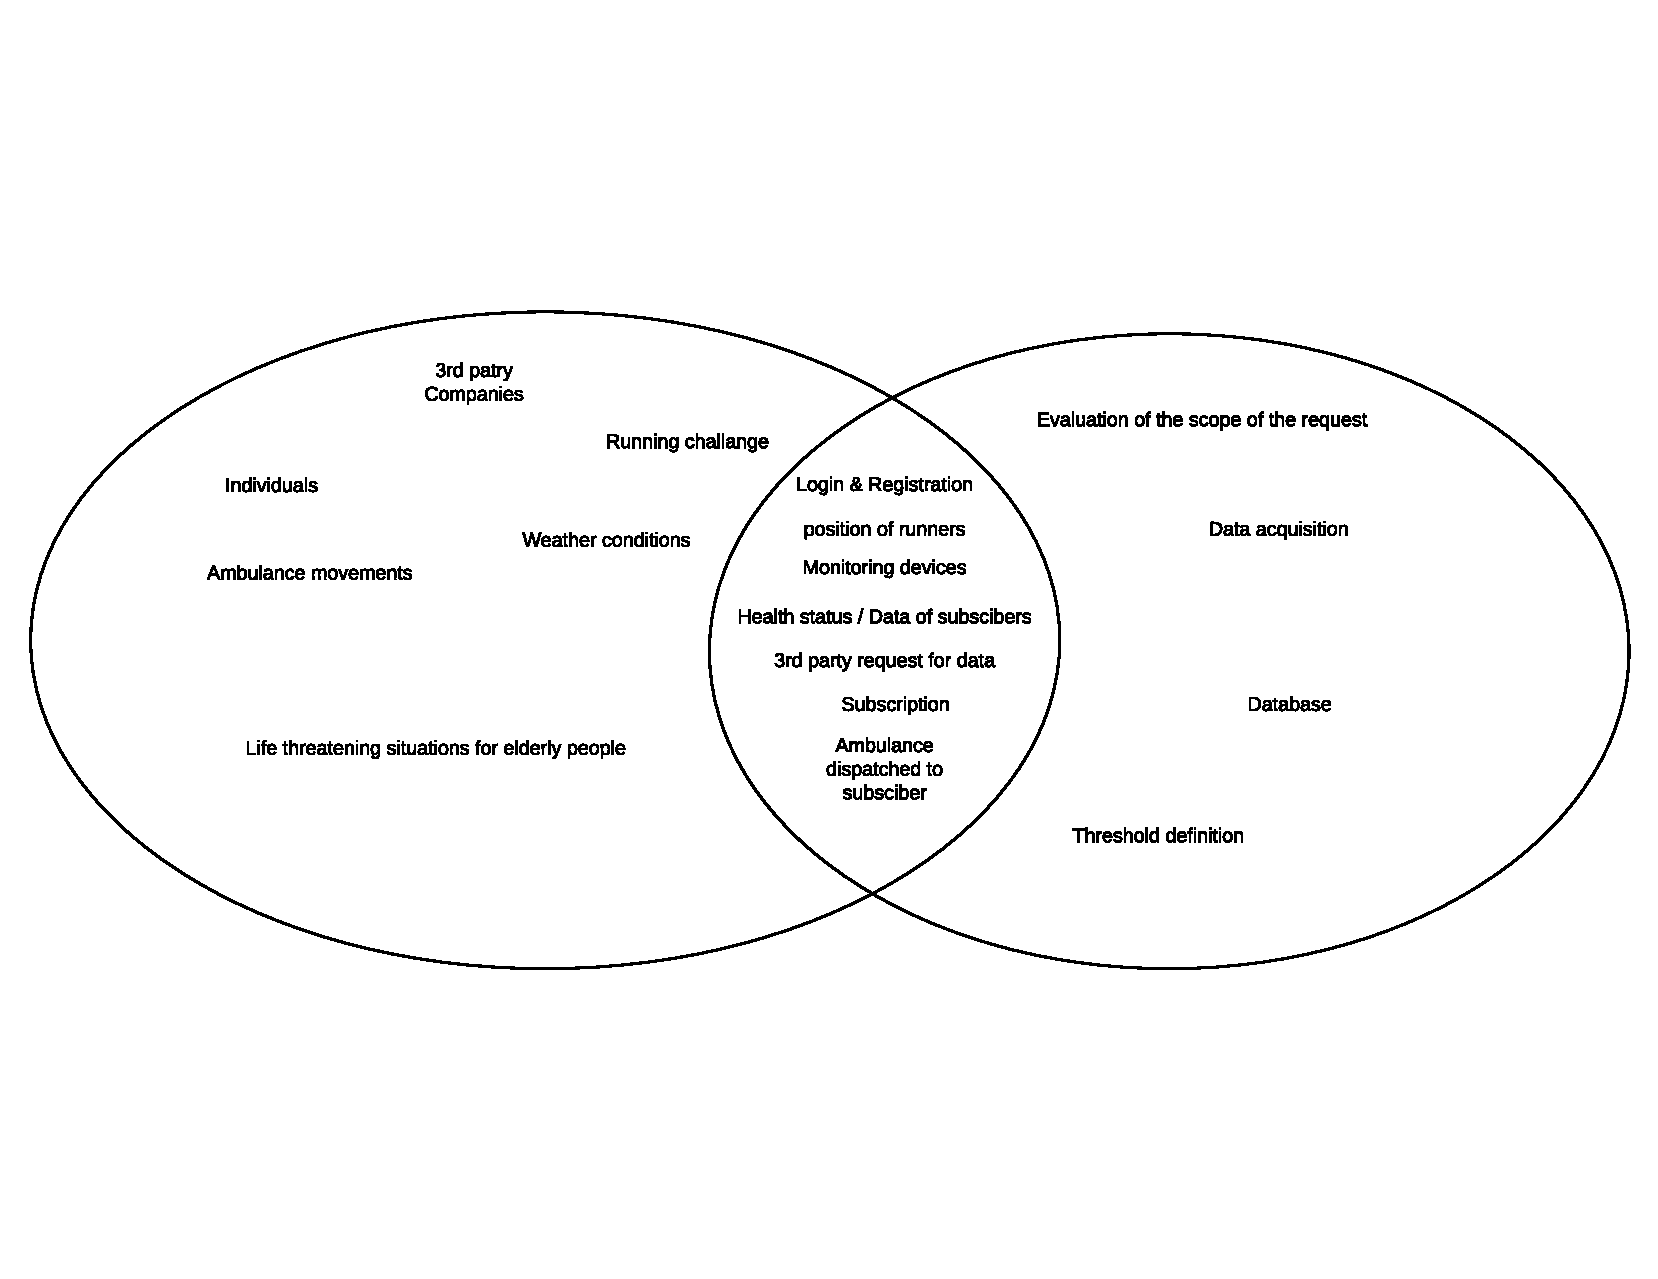
\includegraphics[height=8cm,keepaspectratio]{assets/twatm.pdf}
\end{center}

The system-to-be uses 3 components with different roles in order to work:
\begin{itemize}
    \item \textbf{Data4Help SmartWatch App}: Acquires the data from the smartwatch sensors (heart rate, sleep quality, position, phisical activities) and sends them via Bluetooth to the Data4Help Mobile App
    \item \textbf{Data4Help Mobile App}: Gathers data from the smartwatch, shows various statistics, and sends them to the Data4Help Core Database. Each user can choose which service subscribe to
    \item \textbf{Data4Help Website}: Gives third-party companies the ability to request data, either anonymized or user specific. Moreover, it allows run organizers to define the path of the run and the spectators to see the position of all runners on a map.
    \item \textbf{Data4Help Core}: is intended to connects all other components together providing the logic of the application. It is also responsible for the acceptance of all third-parties requests of data. It also evaluate health status of individuals deciding whether is at risk or not.
\end{itemize}

The list below shows the main goals the system should be able to accomplish:

\begin{itemize}
    \item \textbf{G1}: The system should be able to read sensor data from smart devices.
    \item \textbf{G2}: The system should be able to show acquired data via the Mobile App and the Website.
    \item \textbf{G3}: The system should allow users to register.
    \item \textbf{G4}: The system should allow companies to register.
    \item \textbf{G5}: The system should allow registered companies to request data either from specific individuals or from an anonymized group of individuals.
    \item \textbf{G6}: The system should allow users to accept or decline a company request for their specific data.
    \item \textbf{G7}: The system should provide a payment method to registered companies requesting user data. %eviterei di specificare payment system
    \item \textbf{G8}: The system should be able to communicate directly to ambulances.
    \item \textbf{G9}: The system should be able to react to the lowering of the health parameters below threshold in less than 5 seconds and send the position of the person to the ambulance system. 
    % \item \textbf{G10}: The system should should allow organizers to define the path for the run.
    \item \textbf{G10}: The system should be able to communicate interoperably with its services: \textit{AutomatedSOS} and \textit{Track4Run}
    \item \textbf{G11} The system should allow run organizers to register.
    \item \textbf{G12} If a run organizer is registered, it can define a run i.e. it can define the path that the participants should follow.
    \item \textbf{G13} A user should be able to enroll to a run.
    \item \textbf{G14} Spectators of a run should be able to see each participant's position on a map.
\end{itemize}

%A health data aggregator app that gives the user the ability to monitor all 

%is intended to offer all the functionalities of the service to the individuals, including heart rate monitoring, sleep monitoring




        \subsection{Definitions, Acronyms, Abbreviations}
            \renewcommand{\arraystretch}{1.5}
\begin{center}
    \begin{tabular}{|l|r|}
        \hline
        \textbf{i.e.} & \textit{Id est}, that is  \\
        \hline
        \textbf{w.r.t} & with respect to  \\
        \hline
        \textbf{w.l.o.g.} & without loss of generality \\
        \hline
        \textbf{The company} & TrackMe \\
        \hline
        \textbf{BLE} & Bluetooth Low Energy \\
        \hline
    \end{tabular}
\end{center}
        \subsection{Revision history}
        \subsection{Reference documents}
            \begin{itemize}
\item \textbf{|REFD1|} \href{https://en.wikipedia.org/wiki/Model–view–presenter}{\textbf{MVP}}

\item \textbf{|REFD2|} \href{https://standards.ieee.org/standard/1016-2009.html}{\textbf{IEEE Std 1016-2009 Standard for Information Technology, Systems Design, Software Design Descriptions}}

\item \textbf{|REFD3|} \href{https://it.wikipedia.org/wiki/Representational_State_Transfer}{\textbf{Representational State Transfers}}

\end{itemize}
        \subsection{Document structure}
        This document is divided in the following chapters:
\begin{description}
\item[Implemented requirements] Explains which functional requirements outlined in the RASD are accomplished, and how they are performed.
\item[Design choices] provides reasons about the implementation decisions taken in order to develop the application.
\item[Source code structure] explains and motivates how the source code is structured both in the front end and in the back end.
\item[Testing] provides the main testing cases applied to the the application
\item[REST API] describes the API implemented for the application.
\end{description}
        
    \newpage
    \section{Overall description}
        \subsection{Product perspective}
            Data4Help Core is the central component of the system that connects all the other parts of the structure.
\begin{center}
    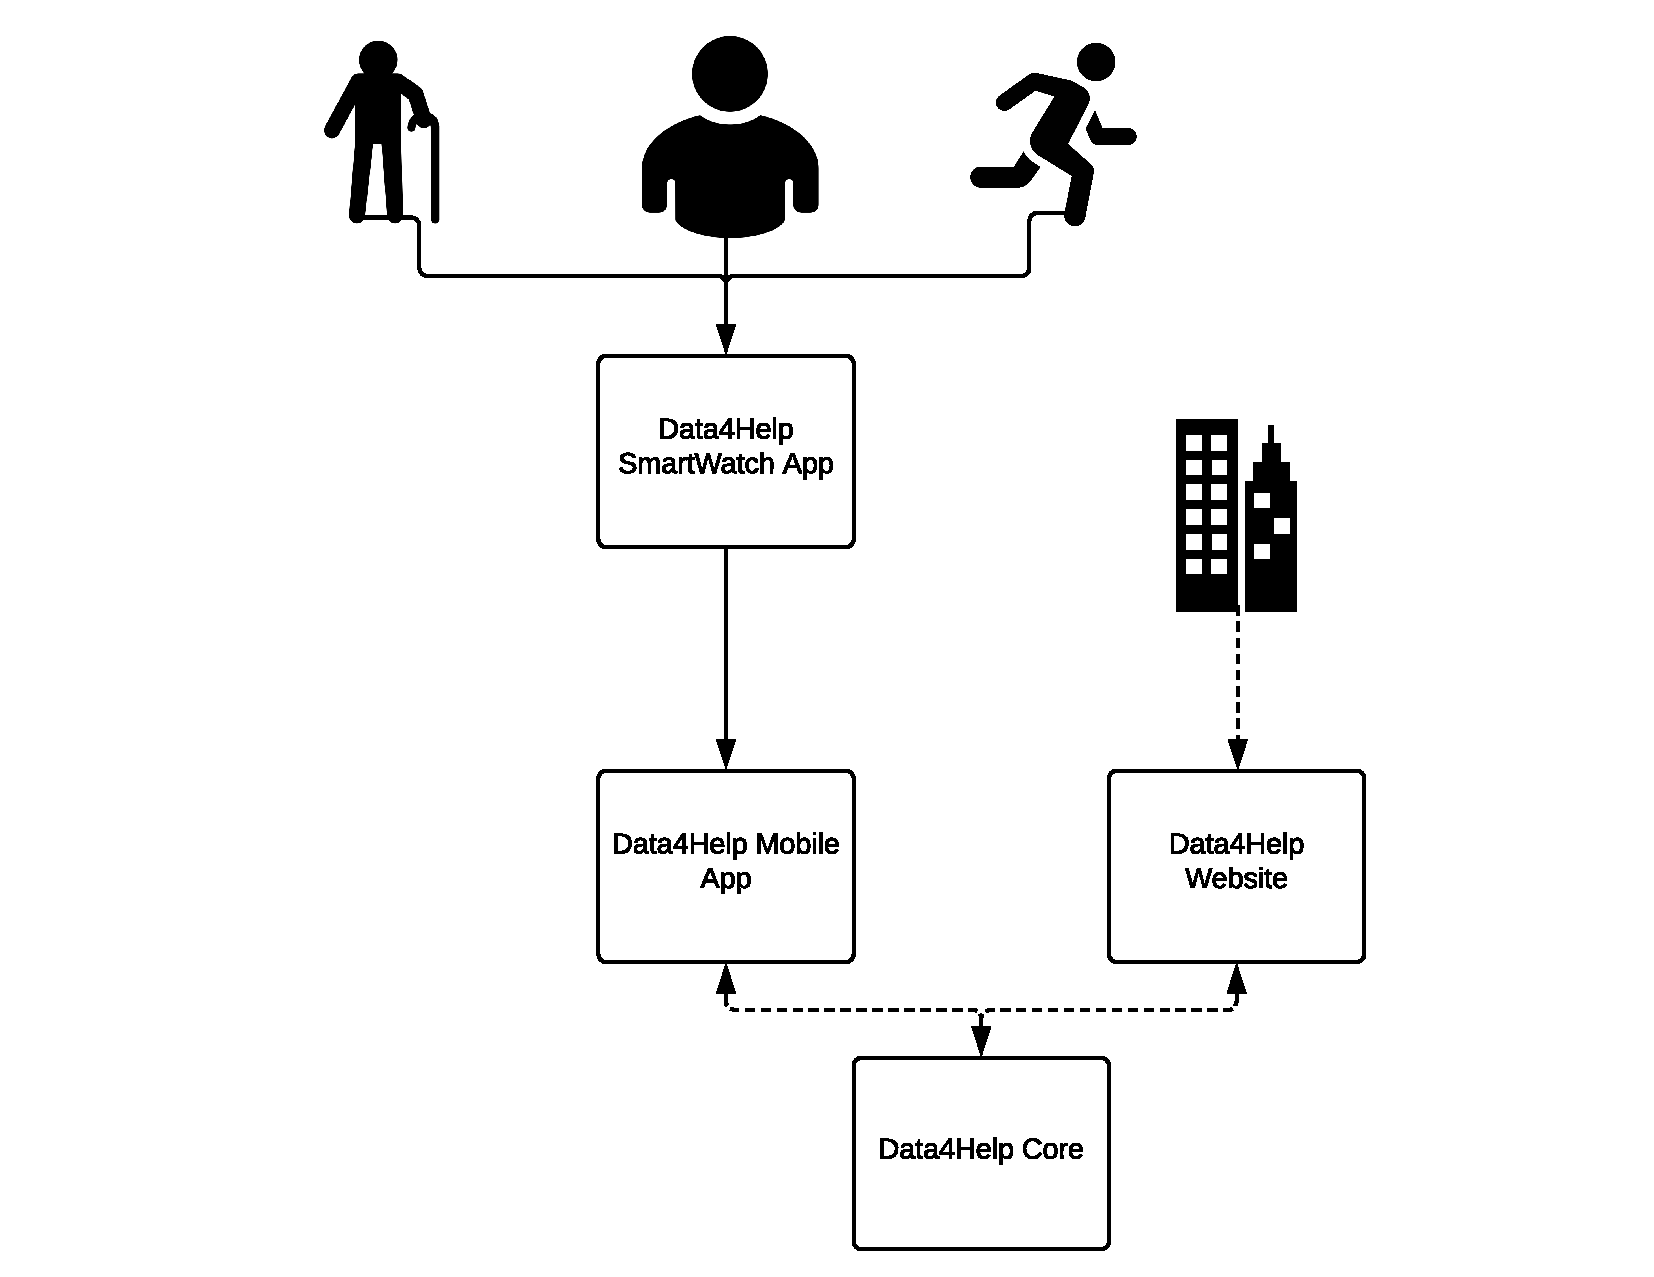
\includegraphics[height=7cm]{assets/useflow.pdf}
\end{center}

The Smartwatch App should be directly connected to the Mobile App to acquire data and let them be shown in the smartphone. In turn, the Mobile App has to communicate with the Data4Help Core that will register the data of the user. The Data4Help Website should communicate with the Data4Help Core as well in order to query directly on the company database.
\newline
\textbf{
TODO: 
A. Product perspective: here we include further details on the shared phenomena and a
domain model (\textbf{class diagrams and statecharts)}
}
        \subsection{Product functions}
            This chapter listing all the functionalities that the system-to-be must offer.
            \subsubsection{Functional requirements}
            Functional requirements for every system component:
\newline
Data4Help Mobile App
\begin{itemize}
    \item Users can register
    \item Users can log-in
    \item Users can only have one account
    \item Logged-in users can edit their account info
    \item Logged-in users can see their data statistics
    \item Logged-in can specify the nature of the daily activities (i.e. running, biking, swimming, hiking)
    \item Logged-in users can edit their account info
    \item Logged-in users can define a path for their running activity
    \item Logged-in users, if subscribed to AutomatedSOS service, can see the monitoring status of their health
    \item Logged-in users, if subscribed to Track4Run service, can register to a run, if organized via the Track4Run service
    \item Logged-in users, if subscribed to Track4Run service, can organize a run
    \item Organizers of a run, if subscribed to Track4Run service, can define the path for that run
    \item Logged-in users can see a run information, if organized via the Track4Run service
\end{itemize}

\noindent Data4Help Smartwatch App
\begin{itemize}
    \item Users can see their health data in real time (i.e heart rate, pressure)
    \item Users can see their sleep monitoring of the previous night
    \item Users can configure the widgets showing their health activity
    \item Users who are participating in a run can see their timing and position through the screen of their Smartwatch, if the run is organized via Track4Run service
\end{itemize}

\noindent Data4Help Website
\begin{itemize}
    \item Companies can register
    \item Companies can log-in
    \item Logged-in companies can see their history and account information
    \item Logged-in companies can subscribe to a payment service of Data4Help
    \item Logged-in companies can update their account information
    \item Logged-in companies can query on some group of individuals data
    previous subscription to an appropriate payment service 
    \item Logged-in companies can access to an individual data, if has the rights to do it (i.e. an Hospital that wants to monitor health status of a patient
    \item Logged-in companies can send support requests
    \item Logged-in companies can export data previously queried using Data4Help
\end{itemize}

\noindent Data4Help Core
\begin{itemize}
\item Can compute queries coming from Webpage component in the TrackMe Database
\item Can charge companies on their payment method respecting Track4Me pricing policy
\item Can access the Track4Me database
\item Can send online notifications  via SMS to all users 
\item Can send online notifications via email to all users
\item Can send online notifications via the Mobile app to its users

\item Can call the Ambulance providing geographical position and critical health parameters to the emergency employee 
\item Can compute for every AutomatedSOS user which are the threshold value to take care of for each health parameter

\item Can detect the geographical position of runners who are using the service Track4Run
\item Can handle run notifications from devices of users using Track4Run (i.e. current runner position and timing)
\end{itemize}

            \subsubsection{Non Functional requirements}
            Non-functional requirements:
\begin{itemize}
    \item Users should be encourages not to be in trouble for being monitored by companies
    \item Users should be encouraged to use the Mobile app with their friends
    \item Users should be encouraged to keep their smart watch all day and all night
    \item Nurse and doctors should encourage their patients to use the Mobile app 
    \item Companies should be encouraged to use the service by other firms
\end{itemize}
            \subsubsection{Company pricing policies}
            The following policies are exclusively referred to the Webpage component services offered to Companies

\begin{itemize}
    \item \textbf{Basic}: The company can query data choosing only from users of one city, one time per day
     \textbf{Price:} 15\euro/month
    \item	\textbf{Basic - Unlimited}: : The company can query data choosing from users of only one city, with no limits
\textbf{Price:} 50\euro/month
    \item \textbf{Medium}: The company can query data choosing only from users of one region of Italy, five times per day
\textbf{Price:} 100\euro/month
    \item \textbf{Medium - Unlimited} The company can query data choosing only from users of one region of Italy, with no limits
\textbf{Price:} 200\euro/month
    \item \textbf{Premium} The company can query data on all Data4Help users, with no limits
\textbf{Price:} 1000\euro/month
\end{itemize}

\noindent Also, companies are also allowed to purchase single queries, with price:

\begin{itemize}
    \item On a city: 5\euro/query
    \item On a region: 20\euro/query
    \item On all users of Data4Help: 50\euro/query
\end{itemize}

\noindent The following policies are exclusively referred to government companies who want to monitor individuals (i.e. hospitals, medical clinics) 

\begin{itemize}
    \item Maximum of 100 patients:
500\euro/month
    \item Maximum of 1000 patients: 
1500\euro/month
    \item No limit on maximum patients:
5000\euro/month
\end{itemize}




\noindent It is not expected to be a pricing policy for Mobile App and Smartwatch App users, which means that the Apps will be free.

\noindent As specified in the Functional requirements, the Data4Help Core component is in charge to calculate the final price for every user using the service.








        \subsection{User characteristics}
            Here is shown the distinction of the users of the Data4Help services.

\noindent The common characteristic for all Customers is that all users of the service must be logged in to use it.
\\
\noindent The users of using all possible components can be distinguished in 2 main categories:
\\
\begin{itemize}
    \item \textbf{Data4Help Individuals Customers}: Users who use the app to take advantage of services offered by it.
    \item \textbf{Data4Help Companies Customers}: Thirty-Party users who can be divided once more in 2 subcategories:
    \begin{itemize}
        \item Companies who wants to use data for marketing purposes
        \item Public companies or clinics who wants to monitor the health status of an individual patient
    \end{itemize}
\end{itemize}






        \subsection{Constraints and dependencies}
            \subsubsection{Constraints}
The constraints for the System-to-be are listed below:
\begin{itemize}
    \item Users are located in Italy
    \item Users must have a Smartwarth and a Mobile phone with a OS compatible with the applications
    \item Users must have Internet connection on their devices
    \item The system must ask the users the permission to store their data following the GDPR policy
    \item The system must ask users to use GPS position on their devices
    \item Companies must have a computer with a compatible browser to use the Data4Help services
\end{itemize}

\subsubsection{Regulatory policies}
As Data4Help will handle sensitive user data (e.g. name, birth date, location, state of health) the Application must treat them respecting the local laws, in particular the GDPR European law. Data attributable to the user must be anonymized in order to appear in a Company's query, unless the user has given explicit authorization to that company.

\subsubsection{Security consideration}
All data transferred between Data4Help Mobile App and Data4Help Core must be encrypted in order to minimize the possibility of a man-in-the-middle attack or any unauthorized access.
For the same reason, all communication between Data4Help Web site and Data4Help Core must be encrypted.
The Bluetooth communication between Data4Help SmartWatch App and Data4Help Mobile app is already encrypted by the Bluetooth stack itself.

\subsubsection{Dependencies}
\begin{itemize}
    \item The system requires a DBMS to store and retrieve data
    \item Maps used by the system to store data relative to geographical position of ther users are provided by external APIs
    \item The system must rely on external Hospitals API in order to call ambulances for \textit{[R9]} of the Core component
\end{itemize}

        \subsection{Assumptions}
            Each part of the system is based on the following domain assumptions.
\begin{itemize}

    \item  D1  The Storage System is reliable.
    
    \item  D2  The SmartWatch on which the \textit{Mobile App} is installed has an accelerometer, a gyroscope, a GPS antenna, and an heart rate sensor and they are always turned on.
    
    \item  D3  Data taken from the previously mentioned sensors are always trusted and consistent.
            
    \item  D4  The user keeps the SmartWatch on his/her wrist during day and night.
    
    \item  D5  The user has a valid Fiscal Code or Social Security Number, and it is unique.
             
    \item  D6  GPS signal is stable, hence the user position is always correct.

    \item  D7  The phone on which the app will be installed has an internet access.

    \item  D8  Every company willing to buy or subscribe to data has a credit card.

    \item  D9  Users of \textit{Automated SOS} have a stable internet connection.
    
    \item  D10  Every Hospital in which the \textit{AutomatedSOS} service is active has an \textit{API} to call the ambulances.
    
    \item  D11  The Hospital \textit{API} service is active 24/7.
    
\end{itemize}
        
    \newpage
    \section{Specific requirements}
         
        \subsection{External Interface Requirements}
          \subsubsection{User Interfaces}
                \textbf{Data4Help Mobile App:}

\textbf{TODO : ADD MOCKUPS! BOTH MOBILE PHONE AND SMARTWATCH} \newline
The Mobile app should offer an easy interface aiming a user friendly experience of the customers. If should be possible to open a menu to navigate through the sub-sections. All the main functions (i.e. see history of activities, see account information) should be easy to access from any sub-section of the app. 
Descriptions of the pages has to be brief and concise.
To see the details of the statistics there should be an info button that shows detailed description about the related data.
If subscribed to the AutomatedSOS service, there should be a page showing the active controls on the user.
In case of using the Track4Run service, there is also the possibility to see the map of a programmed run and seeing on the map all the participants, and their positions. More detailed info of the runners can be shown by tapping on their icon on the map.

The application must follow a proper design for every different mobile operating system:
\begin{itemize}
    \item Android - \vspace{0.3cm} Material Design
    \item iOS - \vspace{0.3cm} Human Interfaces
\end{itemize}
The application should support all the screen resolutions available and optimize the item placement on the screen in the same way for every compatible device.
\newline
The user can configure the graphic of the widget visible from the Smartwatch only using the Mobile App component.



\textbf{Data4Help SmartWatch App} :
The Smartwatch app should provide \textbf{widgets} that let the customer see their daily activity.
There should be one widget for every type of data acquired by the device:
\begin{itemize}
    \item Sleep monitoring 
    \item Heart rate
    \item Blood pressure
\end{itemize}
The user can receive notifications about his activities in the Smartwatch and delete them through it.
\newline

\textbf{Data4Help WebSite}: The Website should offer an easy interface aiming a user friendly experience for the subscribed companies. The main menu should be visible on the top of the page, and must be used to navigate through the sub-sections. All the main functions (i.e. acquired data, account information, etc) should be accessible from any sub-section of the web page. 
Descriptions of the pages have to be clear and exhaustive.
\newline

\textbf{Data4Help Core:} This component does not have a user interface since it is intended to be accessible only by the qualified staff that manages it. 
            \subsubsection{Hardware Interfaces}
                \textbf{Data4Help Mobile App:} The application should require the location services in order to work. If GPS is unavailable on the mobile phone, it can be requested to the Smartwatch app and viceversa. If both unavailable, the application wouldn't work and show an error window to notify the user.
The app should also require a connection from either mobile network or Wi-Fi, but is sufficient to turn it at least once per day. If not, the app will notify the user asking to turn on connectivity. 

\textbf{Data4Help SmartWatch App:} As written for Data4Help Mobile app, but also requires Bluetooth connectivity. If not available, an error message will appear on the Mobile app.

\textbf{Data4Help WebSite:} There is not any special hardware interface needed for the WebSite component.

\textbf{Data4Help Core:} There is not any special hardware interface needed for the Core component.
            \subsubsection{Software Interfaces}
                \begin{itemize}
    \item \textbf{Data4Help SmartWatch App}: Development will focus on the production of a WatchOS and a WearOS app in order to properly communicate with their respective smartphone app.\newline As an app built for the latest version of those OSes is also backwords compatible with their previous versions, there are no particular \textit{minimum version} requirements.
    By developing an app for WatchOS and WearOS, the app will reach the 84\% of all available Smartwatches.

    \item \textbf{Data4Help Mobile App}: Due to the fact that iOS and Android are the only OSes that provide a seamless integration with their smartwatch counterparts, the app will be developed for those platforms only.
    In order to support smartwatch communication there is a minimum version required for those OSes, namely:
    \begin{itemize}
        \item Android \textgreater \vspace{0.1cm} 4.4 (API level 19) (about 94,7\% of devices)
        \item iOS \textgreater \vspace{0.4cm} 9.3 (about 96,3\% of devices)

    \end{itemize}
    
    \item \textbf{Data4Help Website}: It will require the use of a modern Web Browser to be accessed. It will work either on desktop and mobile Web Browsers.
    
    \item \textbf{Data4Help Core}: As the \textit{Core} component will need only to provide \textbf{REST} endpoints for the communication (with ambulance, Website, App) there are no specific requirements on this component.
\end{itemize}

            \subsubsection{Communication Interfaces}
                
In the system there are 2 types of communication.
\begin{enumerate}
    \item The Mobile App and the Web Site need a bidirectional channel with the Core component of the system to operate properly. \\
    This can be achived by providing a REST API on the \textit{Data4Help Core} component.
    
    \item The Smartwatch App needs a direct connection with the Mobile app to give it user's data.\\ The communication between the smart device and the smartphone is achieved via \textit{BLE} and, once the channel is established, the Smartwatch App sends JSON messages to the Mobile App concerning all activities performend from the last syncronization.

\end{enumerate}

\begin{center}
    \begin{small}
    \begin{verbatim}
    {
        userId: "ka8c57pno3",
        last_synchronization: "1512518400",
        heart_rate: {
            "1512518400": 60,
            "1512519000": 61,
            ...
        },
        activities: {
           "1512518400": {
                "_lat": "",
                "_long": ""
            },
            "1512519000": {
                "_lat": "",
                "_long": ""
            },
            ...
        }
    }
    \end{verbatim}
    \end{small}
\end{center}

%% Reference Document
%% https://developer.android.com/guide/topics/connectivity/bluetooth

            \subsubsection{Memory Constraints}
                \begin{itemize}
    \item \textbf{Data4Help SmartWatch App} As the devices on which the app will run have generally less than 1GB of RAM and less than 16GB of non volatile storage the smartwatch app should offload all the unnecessary computations to the mobile app, therefore reducing it size (which could be kept under 10MB) and its memory footprint.
    \item \textbf{Data4Help Mobile App} Based on the functionalities it will provide, the overall size of the app should not exceed 50MB, without taking into account the saved user data.
    \item \textbf{Data4Help Core} The server on which the \textit{Core} component will run will need at least 2GB of RAM and 250MB of non volatile storage in order to host the application. An additional 2TB of storage should be added in order to retain the user-generated data. \newline An estimate on the number of users using the service will suggest at least 64GB of RAM in order to ensure responsive operations for all the services provided.
    \item \textbf{Data4Help Website} The server on which the \textit{Website} will be hosted will need at least 500M of RAM and 50M of non volatile storage in order to store all the assets the website needs.
    To ensure faster response time for all users a minimum of 16GB of RAM would be required.
    
\end{itemize}

% Add refd https://docs.oracle.com/cd/E19226-01/820-7688/abpaj/index.html ??
            
        \subsection{Functional requirements}
            \input{chapters/3.2.FunctionalRequirements.tex}
        \subsubsection{Scenarios}
            Here there are shown some scenarios to better understand the system usage from multiple viewpoints.

\paragraph{Scenario 1} \textbf{ User registration and log-in} \newline
Pierluigi is a Runner, he runs at least once per day and is very focused on the performance he gets during the training session.
In order to do so, he downloaded the Data4Help App  both on Smartwatch and mobile phone, so he registered, confirmed his email address, and then inserted personal data such as Age, Nationality, City of residence and the sport activity he practices.
Once having completed the subscription, he logs in through the Mobile app, turns on Bluetooth on smartphone and smartwatch and the Data4Help apps automatically synchronize in both devices. He sets “running activity” function on Mobile app and starts the run.



\paragraph{Scenario 2} \textbf{ User parameter consulting} \newline
Matteo uses Data4Help mobile app to track his sport activity. When he wants to see the old data from the Mobile app, he opens it, clicks on "Show past activity", inserts the date he's interested in, so the app shows all the activity data for that date from 0:00 to 24:00.


\paragraph{Scenario 3} \textbf{Data synchronization between devices} \newline
Letizia has just finished her Parkour lesson at Milano Gravity sports center.
She would like to see the calories she consumed, the maximum heart-bpm and other health parameters. Luckily, she has a Smartwatch with the Data4Help application installed. First, she turns on the Bluetooth on her smartphone. It automatically synchronizes the data with the smartwatch app, then she opens the Data4Help mobile app and gives a look on the recent statistics.



\paragraph{Scenario 4} \textbf{Hospital registration and purchase } \newline
Villa Serena is a hospital in Jesi trying to introduce an experimental way of monitoring its patients. In order to do so the director of the clinic goes to the website of the Data4Help services, subscribes using the email of the institution, clicks on “Subscribe to a Premium service” choosing the 1000-patients option. Then he adds a payment method and completes the operation.



\paragraph{Scenario 5} \textbf{Patient registration} \newline
Dr. Verdi is a private dermatologist in Milan who wants to use Data4Help in order to monitor his patients. He has already chosen to the  subscription plan with a limit of 100 patients. He asked Maria, one of his patients, to download the Mobile app and subscribe to the service.
Maria subscribes using her e-mail and fiscal code and then communicates her email to the Doctor who immediately adds Maria as her patient. Maria receives a notification asking if she agrees to be monitored by dr. Verdi (identified by his email) and she clicks on ‘accept’.



\paragraph{Scenario 6} \textbf{Company subscription and purchase} \newline
Clear-Water Spa is a company specializing on producing energy drinks for runners that wants to start a marketing campaign in Milan. In order to know where people usually do activities in Milan, it decides to subscribe to Data4Help services. The Marketing director goes to the Web page, subscribes to the service using e-mail and fiscal code, inserts a payment method and purchases the 1-City unlimited query option, specifying “Milan” as the city of preference.
Then he does his research on the city, inserting:
\begin{itemize}
    \item Age of the people to search (i.e. from 20 to 25 year old)
    \item The hour when to search people (i.e. from 9.00 to 10.00)
    \item The health parameter filters (i.e. heart rate $<$ 100 bpm, pressure $>$ 130 mmHg)
\end{itemize}
 The Data4Help system checks if the inquiry is satisfactory (i.e. whether it is too specific), if yes it shows a map with most frequent places of Milan where people go and an average of every health parameter, basing on the data provided by its users. 



\paragraph{Scenario 7}Subscription for the "Automated SOS" service \newline
Ottavio is a patient of Dr. Verdi using AutomatedSOS services offered by the Data4Help mobile app. The smartwatch of Ottavio has detected that his health parameters have gone below the threshold calculated by Data4Help, so the service is immediately notified and calls the ambulance of the closest hospital to the patient. The hospital receives the emergency notification  and sends an ambulance  to the position of Ottavio.


\paragraph{Scenario 8} Organizing a race \newline
Luigi is a race organizer for a famous sports brand in Milan. He wants to use the services offered by Track4Run in order to attract more runners, so first he goes to the Data4Help Mobile App and registers inserting his name, surname, email, Fiscal Code and specifying he is a Run organizer. After consolidating his email, he log in through the mobile app and clicks “Organize a new running event”. He fills in a module specifying the city of the race, the date, the starting time, the length in km and a description. Once finished, he clicks on “post the running event” and obtains a link where he can see all the details of the joining participants.



\paragraph{Scenario 9} A runner registers and starts the activity \newline
Salvatore is a professional runner of Milano.  He has recently been searching for some running events in order to test his performances, so he opens Data4Help app on his smartphone and clicks on “\textit{See the closest running event}”.
He is shown a map with all the races of Milan starting that day. Salvatore clicks on the closest one and a window appears on the screen of the app showing all the relevant data. Then he decides to join the race, so he clicks on “join the running event”. After that he receives the race number and a confirmation e-mail.



\paragraph{Scenario 10} Viewers of a race use the Data4Help mobile app \newline
Amanda and Dario have a son, Roberto, who has just joined a race organized through the Data4Help app. Since Roberto’s family wants to know their son geographical position during the race, they also download the app on their smartphones and register, specifying they are “\textit{spectators of a running event}”. Then they log in, click on “\textit{See nearby running events}”, choose the race they are interested in and click on “\textit{See runners}”. A map showing the position of all runners marked with blue points appears on the screen. The parents type the name of their son on the search box of the app and  his location becomes red and can be tracked.

            
        \subsubsection{Requirements mapping}
            In the following section are explained the functional requirements of the application, grouped under each goal.

\begin{itemize}
    \item \textbf{G1}: The system should be able to show acquired data via the Mobile App and the Website.
    \paragraph{Requirements}
   \begin{itemize}
    \item \textbf{[R1$_S$]}: App can read data from sensor and store it locally.
    \item \textbf{[R2$_S$]}: App can send data registered locally to Data4Help Mobile App
   \end{itemize}
   \paragraph{Domain assumptions}
   \begin{itemize}
    \item  \textbf{D1}  The Storage System is reliable.
    
    \item  \textbf{D2}  The SmartWatch on which the \textit{Mobile App} is installed has an accelerometer, a gyroscope, a GPS antenna, and an heart rate sensor.
    
    \item  \textbf{D3}  Data taken from the previously mentioned sensors are always trusted and consistent.
            
    \item  \textbf{D4}  The user keeps the SmartWatch on his/her wrist during day and night.
   \end{itemize}
   
    \item \textbf{G2}: The system should allow users to register by providing his Fiscal Code or his Social Security Number, an username and a password.
    \paragraph{Requirements}
   \begin{itemize}
    \item \textbf{[RM$_M$]}: Users can register, after providing a username, a password and a Fiscal Code/Social Security Number and have connected a compatible Smartwatch
    \item \textbf{[R14$_C$]}: Can validates information provided by the user during registration
   \end{itemize}
   \paragraph{Domain assumptions}
   \begin{itemize}
    \item  D5  The user has a valid Fiscal Code or Social Security Number, and it is unique.
   \end{itemize}
   
    \item \textbf{G3}: The system should allow companies to register.
    \paragraph{Requirements}
   \begin{itemize}
    \item \textbf{[R1$_W$}: Companies can register, after providing a username, a password and a payment method
    \item \textbf{[R14$_C$]}: Can validates information provided by the user during registration
   \end{itemize}
    \item \textbf{G4}: The system should allow registered companies to request data from an anonymized group of individuals, only if individuals in the group are more than 1000.
    \paragraph{Requirements}
   \begin{itemize}
    \item \textbf{[R2$_S$]}: App can send data registered locally to Data4Help Mobile App
    \item \textbf{[R5$_C$]}: Can receive and store health parameters and geographical position of registered users
    \item \textbf{[R7$_C$]}: Can execute queries of companies checking if the searches involve more than 1000 anonimyzed users
   \end{itemize}
   \paragraph{Domain assumptions}
   \begin{itemize}
    \item  D1  The Storage System is reliable.
   \end{itemize}
   
    \item \textbf{G5}: The system should allow registered companies to request data from an individual person, only if individuals accept the request.
    \paragraph{Requirements}
   \begin{itemize}
      \item \textbf{[R6$_C$]}: Can execute queries of companies on individuals if the user has accepted the monitoring request from the company
      \item \textbf{[R1$_C$]}: Can send online notifications via SMS to all users 
    \item \textbf{[R2$_C$]}: Can send online notifications via email to all users
    \item \textbf{[R3$_C$]}: Can send online notifications via the Mobile app to its users
   \end{itemize}
    
    \item \textbf{G6}: The company should be able to pay through the system in order to buy data queries/subscribe to plans.
    \paragraph{Requirements}
   \begin{itemize}
       \item \textbf{[R4$_W$]}: Logged-in companies can subscribe to a payment service of Data4Help
       \item \textbf{[R15$_C$]}: Can charge companies on their payment method respecting Track4Me pricing policy
   \end{itemize}
   \paragraph{Domain assumptions}
   \begin{itemize}
       \item  D8  Every company willing to buy or subscribe to data has a credit card.
   \end{itemize}
   
    \item \textbf{G7}: The system should allow a company to subscribe to new data and receive them as soon as they are produced.
    \paragraph{Requirements}
   \begin{itemize}
       \item \textbf{[R6bis$_W$]}: Logged-in companies can subscribe to a query data
       \item \textbf{[R2$_C$]}: Can send online notifications via email to all users
   \end{itemize}
   \paragraph{Domain assumptions}
   \begin{itemize}
        \item  D1  The Storage System is reliable.
    
        \item  D2  The SmartWatch on which the \textit{Mobile App} is installed has an accelerometer, a gyroscope, a GPS antenna, and an heart rate sensor and they are always turned on.
    
        \item  D3  Data taken from the previously mentioned sensors are always trusted and consistent.
   \end{itemize}
   
    \item \textbf{G8}: The system should be able to monitor user's health parameter.
    \paragraph{Requirements}
   \begin{itemize}
       \item \textbf{[R1$_S$]}: App can read data from sensor and store it locally.
        \item \textbf{[R2$_S$]}: App can send data registered locally to Data4Help Mobile App
        \item \textbf{[R4$_C$]}: Can save and store permanently user data
    \item \textbf{[R5$_C$]}: Can receive and store health parameters and geographical position of registered users

   \end{itemize}
   \paragraph{Domain assumptions}
   \begin{itemize}
    \item  D1  The Storage System is reliable.
    
    \item  D2  The SmartWatch on which the \textit{Mobile App} is installed has an accelerometer, a gyroscope, a GPS antenna, and an heart rate sensor and they are always turned on.
    
    \item  D3  Data taken from the previously mentioned sensors are always trusted and consistent.
            
    \item  D4  The user keeps the SmartWatch on his/her wrist during day and night.
    
     \item  D7  The phone on which the app will be installed has an internet access.
 
   \end{itemize}
   
   
    \item \textbf{G9}: The system should be able to react to the lowering of the health parameters below threshold in less than 5 seconds and send the position of the person to the ambulance system. 
    \paragraph{Requirements}
   \begin{itemize}
    \item \textbf{[R1$_S$]}: App can read data from sensor and store it locally.
    \item \textbf{[R2$_S$]}: App can send data registered locally to Data4Help Mobile App

    \item \textbf{[R5$_C$]}: Can receive and store health parameters and geographical position of registered users

    \item \textbf{[R9$_C$]}: Can communicate directly with the nearest hospital \textit{API}.
    \item \textbf{[R10$_C$]}: Can provide geographical position and critical health parameters to the emergency employee using the \textit{API}
    \item \textbf{[R11$_C$]}: Can compute for every AutomatedSOS user which are the threshold value to take care of for each health parameter

   \end{itemize}
   \paragraph{Domain assumptions}
   \begin{itemize}
    \item  D2  The SmartWatch on which the \textit{Mobile App} is installed has an accelerometer, a gyroscope, a GPS antenna, and an heart rate sensor and they are always turned on.
    
     \item  D3  Data taken from the previously mentioned sensors are always trusted and consistent.
            
     \item  D4  The user keeps the SmartWatch on his/her wrist during day and night.
    
     \item  D7  The phone on which the app will be installed has an internet access.
     
    \item  D9  Users of \textit{Automated SOS} have a stable internet connection.
    
    \item  D10  Every Hospital in which the \textit{AutomatedSOS} service is active has an \textit{API} to call the ambulances.
    
    \item  D11  The Hospital \textit{API} service is active 24/7.
   \end{itemize}
   
   
    \item \textbf{G10} The system should allow run organizers to register.
    \paragraph{Requirements}
   \begin{itemize}
    \item \textbf{[R10$_W$]}: Run organizers can register
    \item \textbf{[R11$_W$]}: Run organizers can login
    \item \textbf{[R14$_C$]}: Can validates information provided by the user during registration
   \end{itemize}
    
    
    \item \textbf{G11} If a run organizer is registered, it can define a run i.e. it can define the path that the participants should follow.
    \paragraph{Requirements}
   \begin{itemize}
    \item \textbf{[R12$_W$]}: Logged-in run organizers can organize a run
    \item \textbf{[R13$_W$]}: Organizers of a run can define the path and additional information for that run
    \item \textbf{[R14$_W$]}: Organizers of a run can start the run
   \end{itemize}
   
   
    \item \textbf{G12} A user should be able to enroll to a run, if he is close to the starting point and has a valid inscription code.
    \paragraph{Requirements}
   \begin{itemize}
    \item \textbf{[R8$_M$]}: Logged-in users can register to a run before the start time
    \item \textbf{[R9$_M$]}: Logged-in users can see a run information
   \end{itemize}

   
   
    \item \textbf{G13} Spectators of a run should be able to see each participant's position on a map.
    \paragraph{Requirements}
   \begin{itemize}
    \item \textbf{[R12$_C$]}: Can compute each athlete's rank in a run and send it to each user device.
    \item \textbf{[R13$_C$]}: Can send the position and rank of athletes during a run to spectator's devices.
   \end{itemize}
   
   
    \item \textbf{G14} Users should be able to log in
    \paragraph{Requirements}
   \begin{itemize}
     \item \textbf{[R1$_M$]}: Users can log-in rank of athletes during a run to spectator's devices.
     
   \end{itemize}
   
       \item \textbf{G15} Companies should be able to log in
    \paragraph{Requirements}
   \begin{itemize}
    \item \textbf{[R12$_C$]}: Can compute each athlete's rank in a run and send it to each user device.
    \item \textbf{[R13$_C$]}: Can send the position and rank of athletes during a run to spectator's devices.
   \end{itemize}
   
       \item \textbf{G16} Run organizers must be able to 
    \paragraph{Requirements}
   \begin{itemize}
    \item \textbf{[R12$_C$]}: Can compute each athlete's rank in a run and send it to each user device.
    \item \textbf{[R13$_C$]}: Can send the position and rank of athletes during a run to spectator's devices.
   \end{itemize}
   
   \end{itemize}

   
   
        
        \newpage
        \subsubsection{Use cases}
            \paragraph{User registration}
\begin{center}
\begin{table}[H]
\centering
\begin{tabular}{l|p{0.7\textwidth}}
\textbf{Actors} & Not registered user, Mobile app, Track4Me core App \\
\textbf{Start conditions} & None \\
\textbf{Event flow}  & 


 \begin{minipage}[t] {0.7\textwidth} 
 \begin{itemize}
      \item  not registered user clicks on “Subscribe”
      \item not registered user inserts an username, an email, a Fiscal Code or SSN and a password
      \item The system checks if username is not used by any other user
      \item The system checks if email is not used by any other user
      \item The system checks if Fiscal Code / SSN is valid
      \item The mobile app checks if a compatible smartwatch is connected and has the Smartwatch Data4Help app installed
      \item The system generates a confirmation mail
      \item The user confirms the registration inserting the code received via email 
      \item The system shows a registration complete screen
  \end{itemize}
\end{minipage}
 \\
\textbf{Exit condition} & User information used for registering are stored in the company database \\
\textbf{Exceptions} & 
\begin{minipage}[t] {0.7\textwidth} 
 \begin{itemize}
 
 \item The username is used by another user
\item The email is used by another user
\item The Fiscal Code/SSN is not valid
\item Smartwatch is not compatible
\item Smartwatch has not Data4Help app installed
\end{itemize}
 \end{minipage}\\
\textbf{Goals} & G2 
\end{tabular}

\end{table}
\end{center}


\begin{figure}[H]
  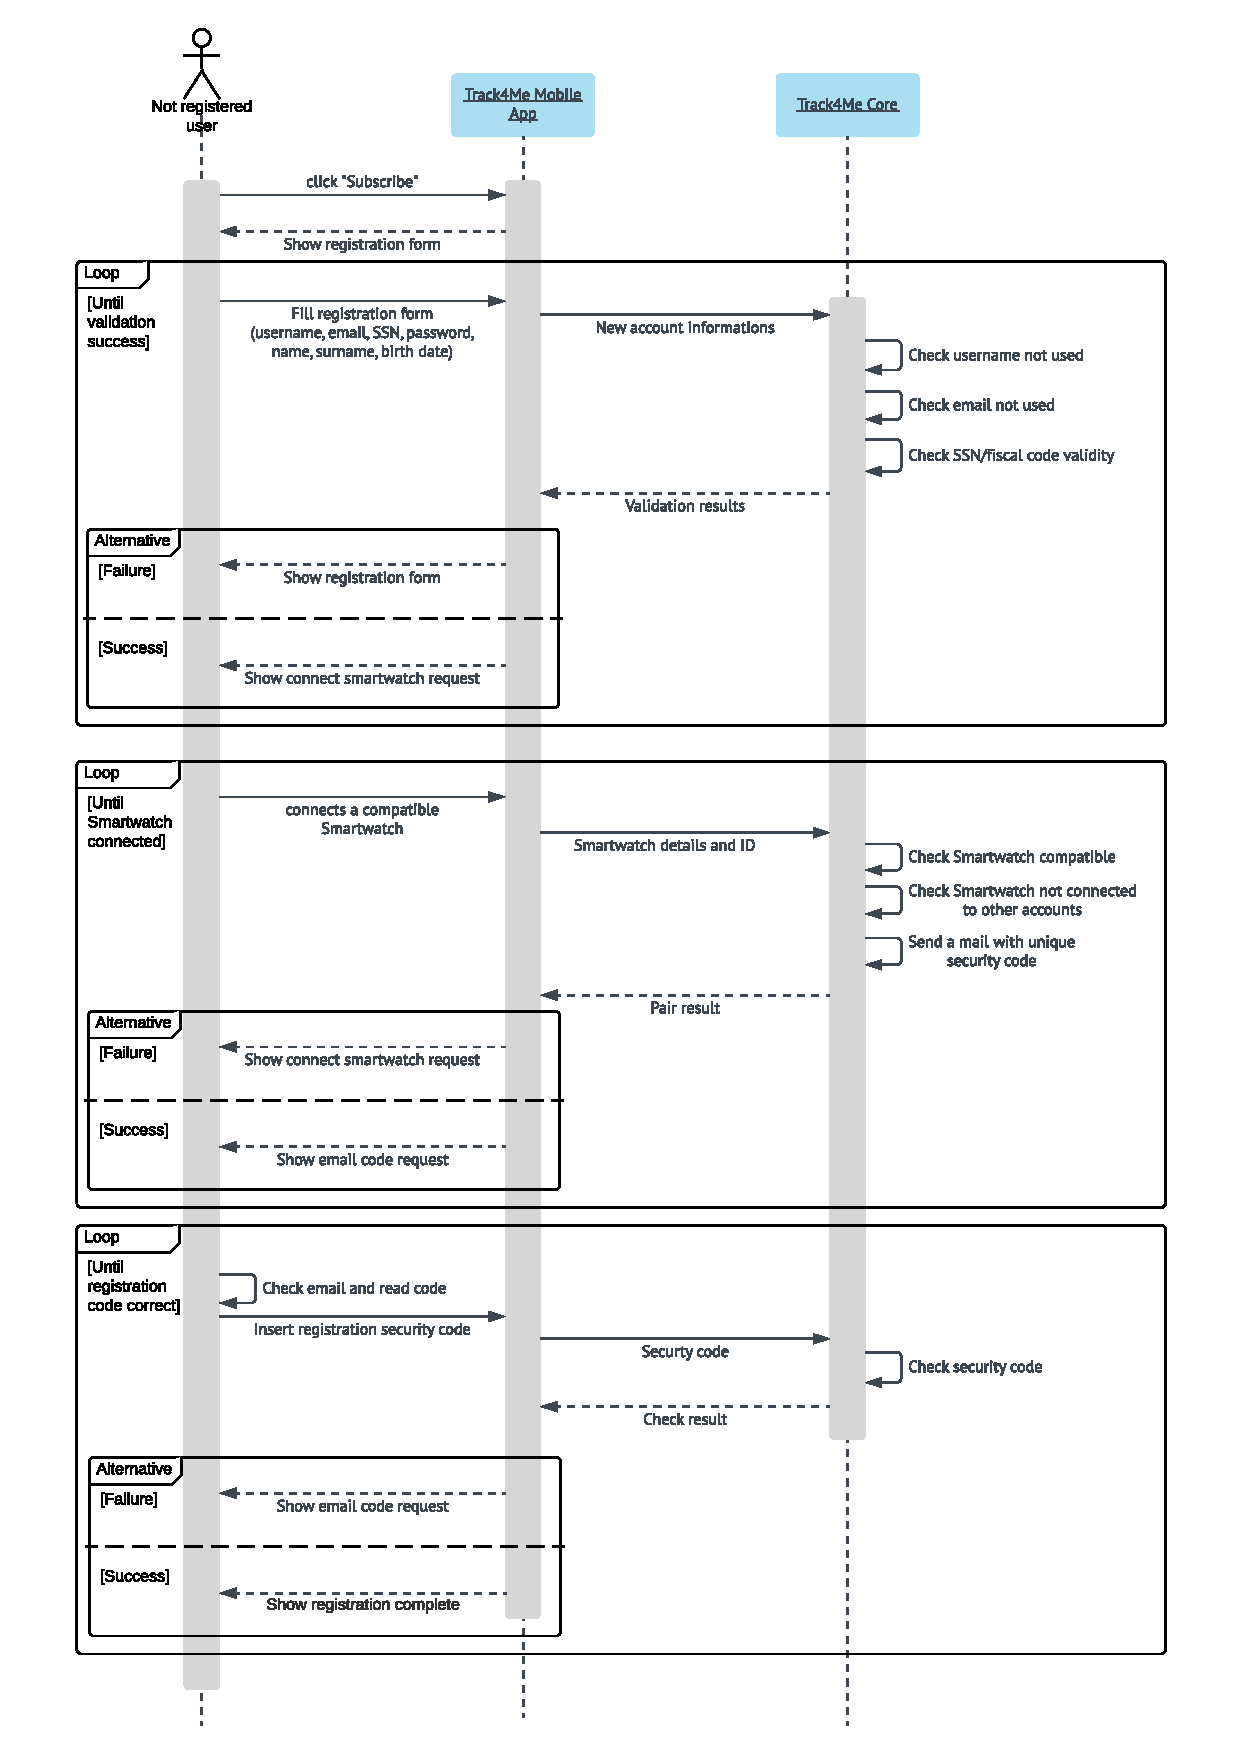
\includegraphics[width=\textwidth,height=\textheight,keepaspectratio]{assets/sequence/UserRegistration.pdf}
  \caption{User registration sequence diagram}
  \label{fig:UserRegistrationSequence}
\end{figure}



\newpage
\paragraph{Consulting of activity history}
\begin{center}
\begin{table}[H]
\centering
\begin{tabular}{l|p{0.7\textwidth}}
\textbf{Actors} & Registered User \\
\textbf{Start conditions} & The user is logged in \\
\textbf{Event flow}  & \begin{minipage}[t]{0.7\textwidth}
    \begin{itemize}
        \item Registered user clicks on “Show past activities” on the Mobile phone
        \item the app shows a screen for searching data information
        \item registered user inserts year, month and the day to search and clicks on the type of data searched
        \item  the system searches for a correspondence in the company database
        \item the system shows a screen showing the required data in a graph
    \end{itemize}
    
\end{minipage}\\ 
    
\textbf{Exit condition} & None \\
\textbf{Exceptions} &  \begin{minipage}[t]{0.7\textwidth}
    \begin{itemize}
        \item The specified day of the calendar is not valid

        \item The specified day of the calendar shows no activities of the user
    \end{itemize}
    
\end{minipage} \\
\textbf{Goals} & \textbf{G1}
\end{tabular}

\end{table}
\end{center}

\begin{figure}[H]
  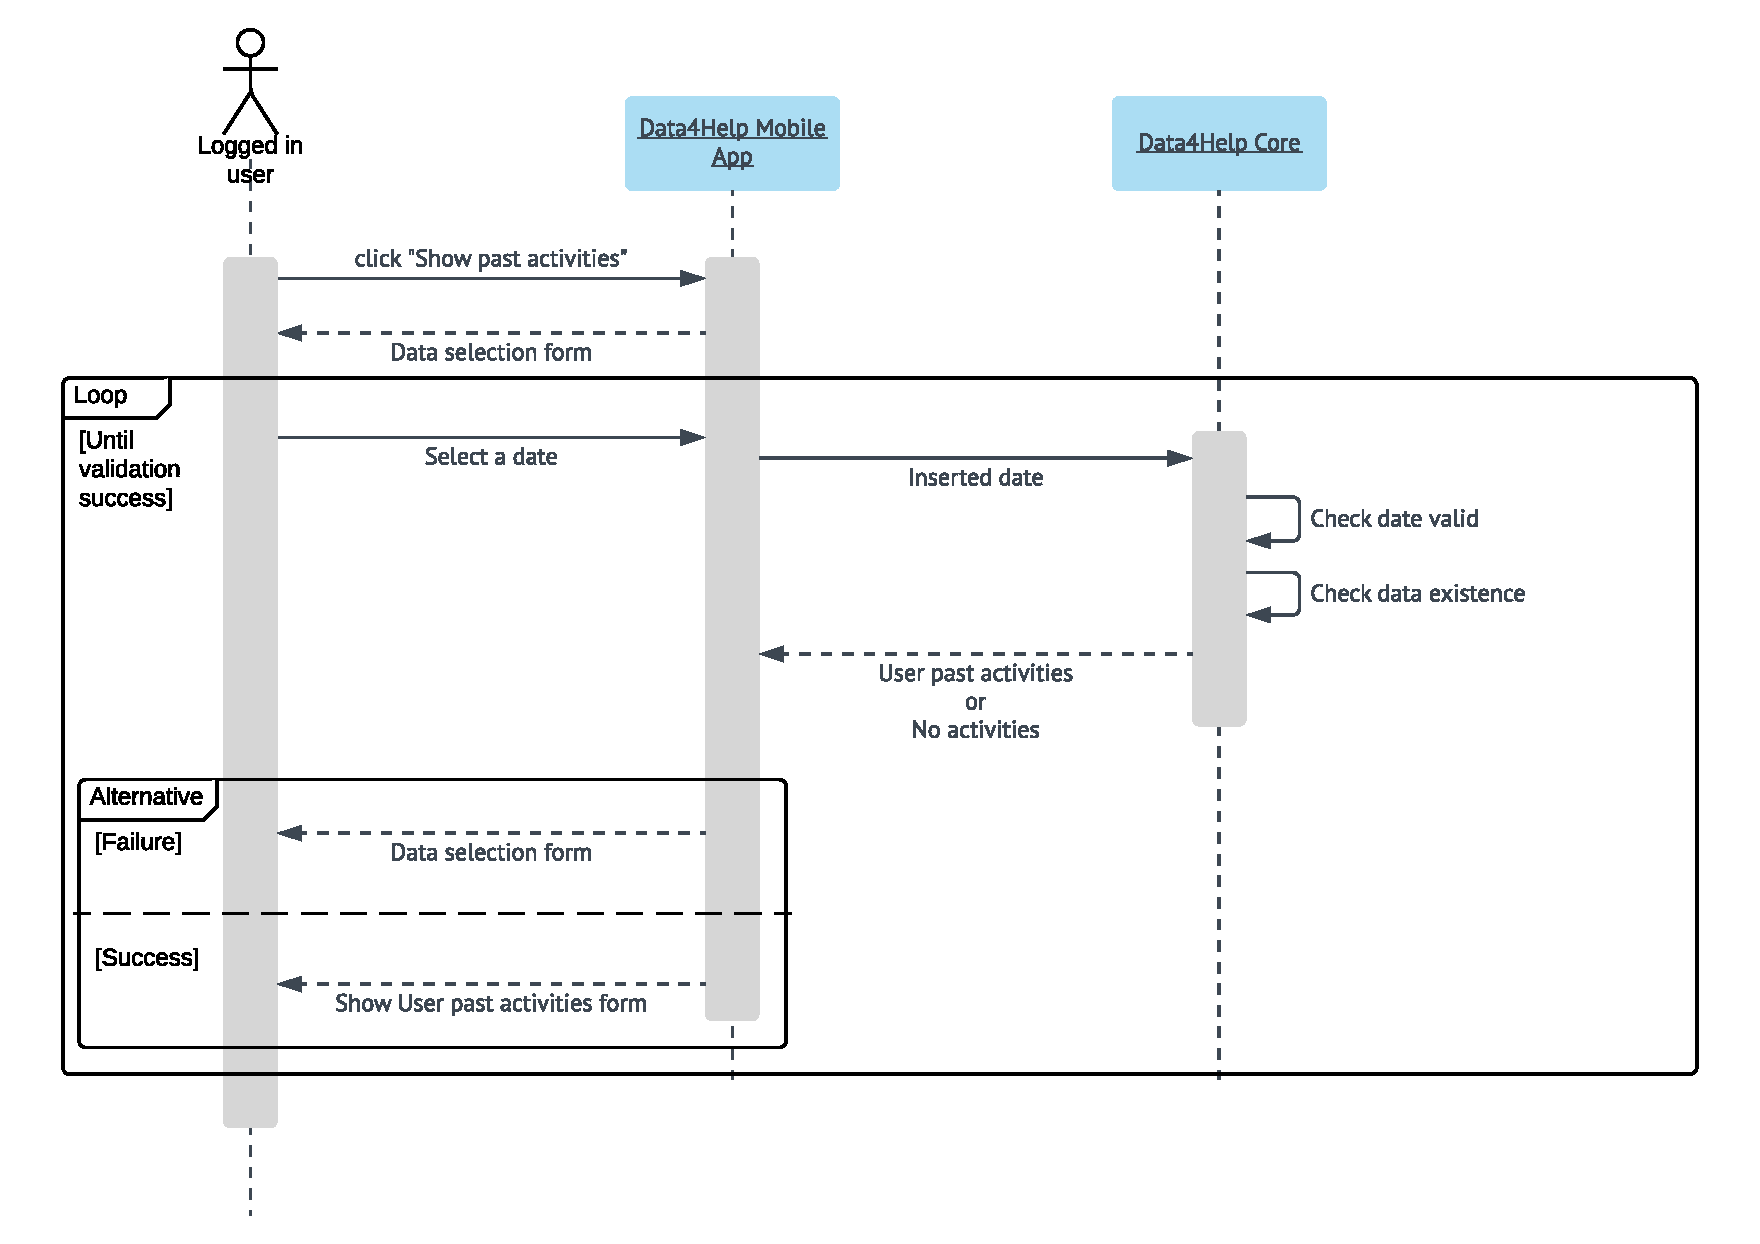
\includegraphics[width=\textwidth,height=\textheight,keepaspectratio]{assets/sequence/ConsultingOfActivityHistory.pdf}
  \caption{Consulting of activity history sequence diagram}
  \label{fig:ConsultingOfActivityHistory}
\end{figure}










\paragraph{Data Synchronization between Smartwatch and Smartphone}
\begin{center}
\begin{table}[H]
\centering
\begin{tabular}{l|p{0.7\textwidth}}
\textbf{Actors} & 
Mobile app, smartwatch app \\
\textbf{Start conditions} & Bluetooth connection enstablished between smartwatch and smartphone \\
\textbf{Event flow}  & \begin{minipage}[t]{0.7\textwidth}
    \begin{itemize}
        \item User turns on Bluetooth of the smartwatch and smartphone


        \item The smartphone requests connection to smartwatch

        \item Smartwatch confirms connection
        \item Smartwatch send data registered in the day 
        \item Smartphone accept data and store locally

    \end{itemize}
    
\end{minipage}\\
\textbf{Exit condition} & Data in the user smartphone is synchronized with data of the smartwatch and stored locally \\
\textbf{Exceptions} & Connection Refused \\
\textbf{Goals} & G1
\end{tabular}

\end{table}
\end{center}

\begin{figure}[H]
  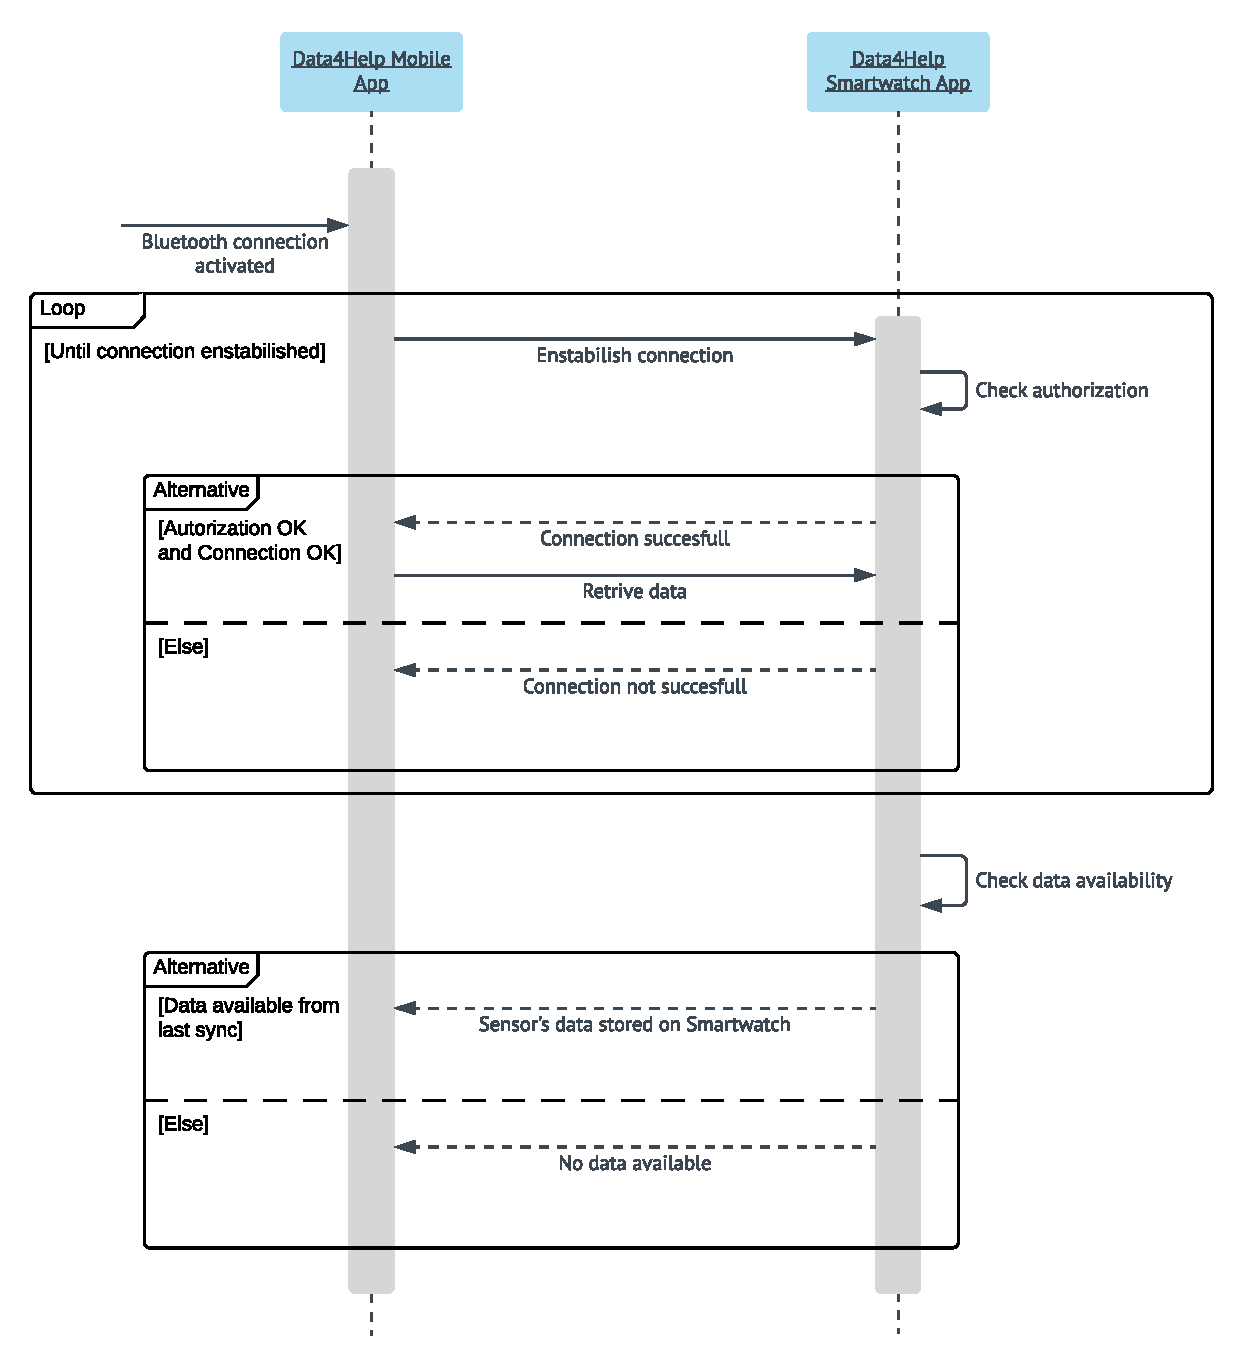
\includegraphics[width=\textwidth,height=\textheight,keepaspectratio]{assets/sequence/DataSynchronizationBetweenSmartwatchAndSmartphone.pdf}
  \caption{Data Synchronization between Smartwatch and Smartphone sequence diagram}
  \label{fig:DataSynchronizationBetweenSmartwatchAndSmartphone}
\end{figure}










\newpage
\paragraph{Company registration}
\begin{center}
\begin{table}[H]
\centering
\begin{tabular}{l|p{0.7\textwidth}}
\textbf{Actors} & Not registered company \\
\textbf{Start conditions} & None \\


\textbf{Event flow}  & \begin{minipage}[t]{0.7\textwidth}
    \begin{itemize}
        \item not registered company clicks on “Subscribe”
\item not registered company inserts a username, an email, a payment method and a password
\item The system checks if email is not used by any other user
\item The system checks if Payment method is valid
\item The system generates a confirmation mail
\item The company confirms the registration click on “Confirm email”
\item The system shows a registration complete screen
    \end{itemize}
    
\end{minipage}\\ 

\textbf{Exit condition} & Company information used for registering is stored in the company database \\
\textbf{Exceptions} & \begin{minipage}[t]{0.7\textwidth}
    \begin{itemize}
        \item The username is used by another company
\item The email is used by another company
\item The Payment method is not valid

    \end{itemize}
    
\end{minipage}\\
\textbf{Goals} & G3 
\end{tabular}

\end{table}
\end{center}

\begin{figure}[H]
  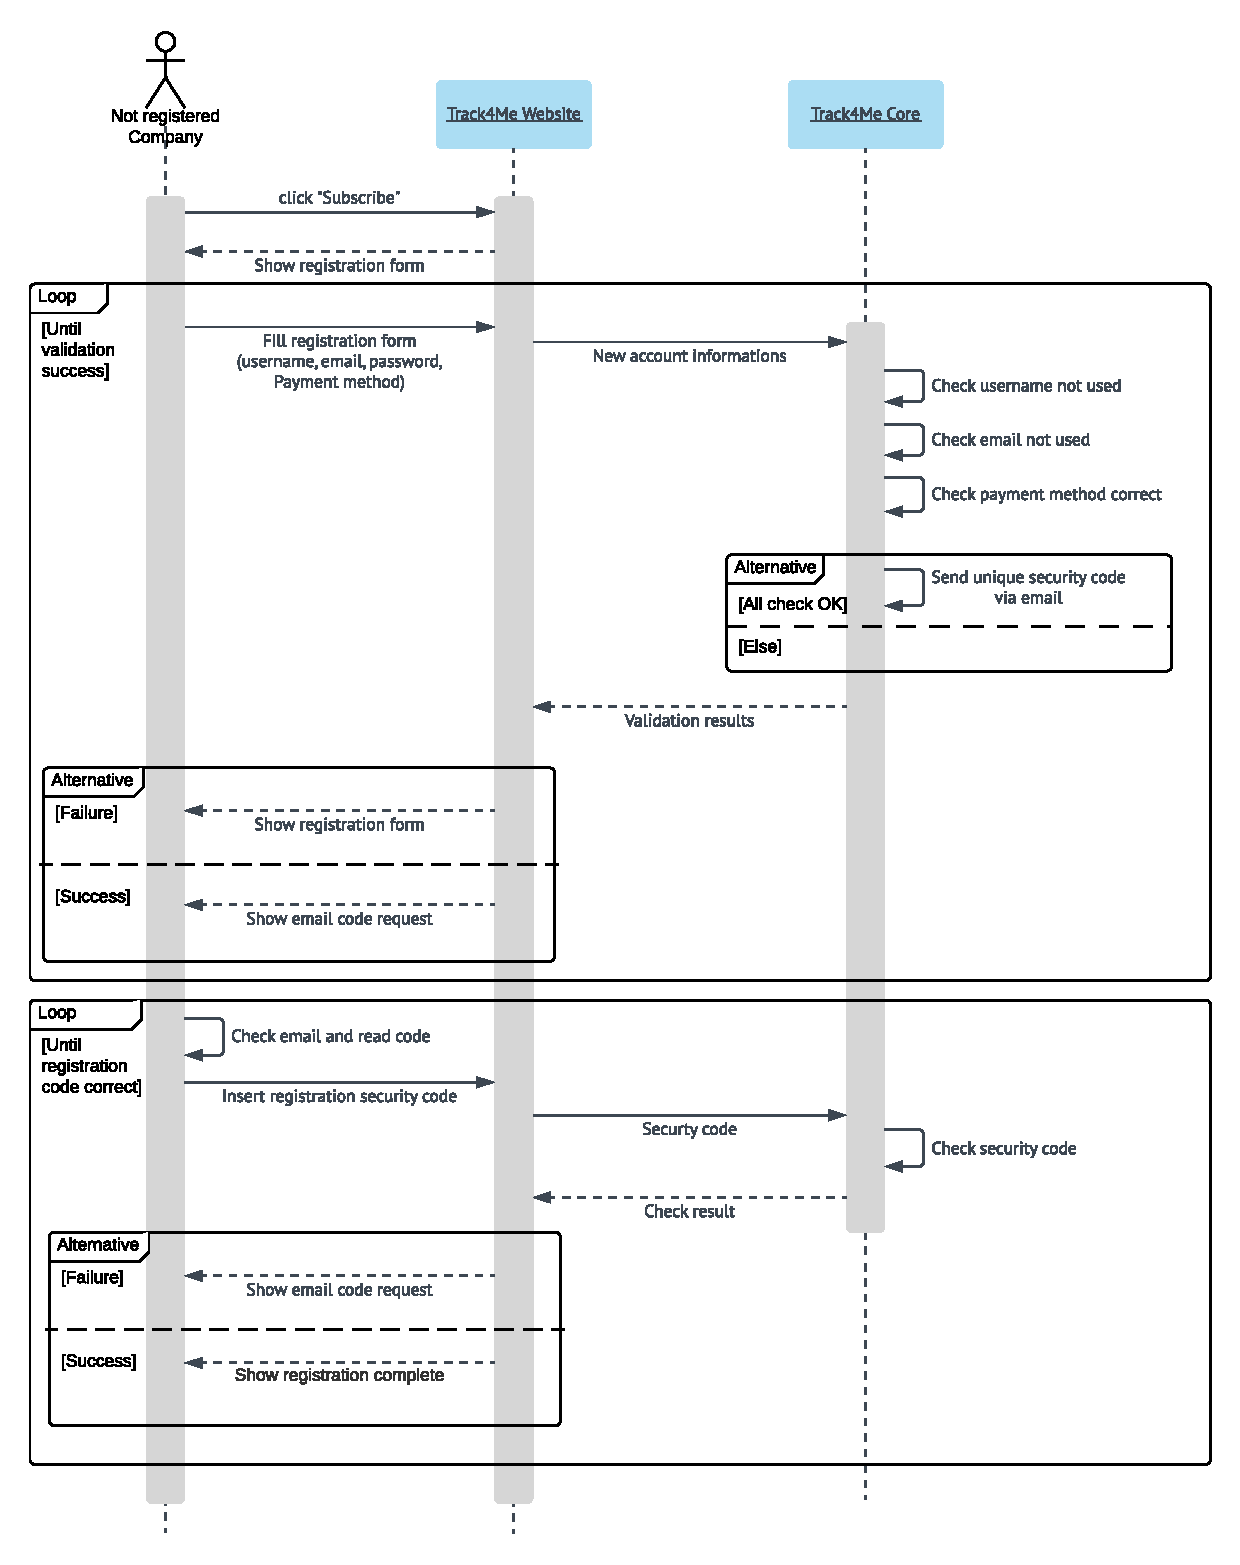
\includegraphics[width=\textwidth,height=\textheight,keepaspectratio]{assets/sequence/CompanyRegistration.pdf}
  \caption{Company registration sequence diagram}
  \label{fig:CompanyRegistration}
\end{figure}











\newpage
\paragraph{Company query search on multiple individuals}
\begin{center}
\begin{table}[H]
\centering
\begin{tabular}{l|p{0.7\textwidth}}
\textbf{Actors} &
Company, WebSite, core component
 \\
\textbf{Start conditions} & None \\
\textbf{Event flow}  &  \begin{minipage}[t]{0.7\textwidth}
    \begin{itemize}
        \item Company clicks on “Start a query” on the website


        \item System checks if the company has query left

        \item System shows the page on the website
        \item Company specifies age of people to search, hours of the day, health parameter filters
 
        \item System validates the request
        \item System send the required data formatted on a pdf page on the website
        \item Company download the data

    \end{itemize}
    
\end{minipage} \\
\textbf{Exit condition} & Query generated as pdf file and stored in the Data4Help database \\
\textbf{Exceptions} & \begin{minipage}[t]{0.7\textwidth}
    \begin{itemize}
        \item No query left for the company type of subscription
        \item Not valid query
    \end{itemize}
    
\end{minipage} \\
\textbf{Goals} & G4
\end{tabular}

\end{table}
\end{center}

\begin{figure}[H]
  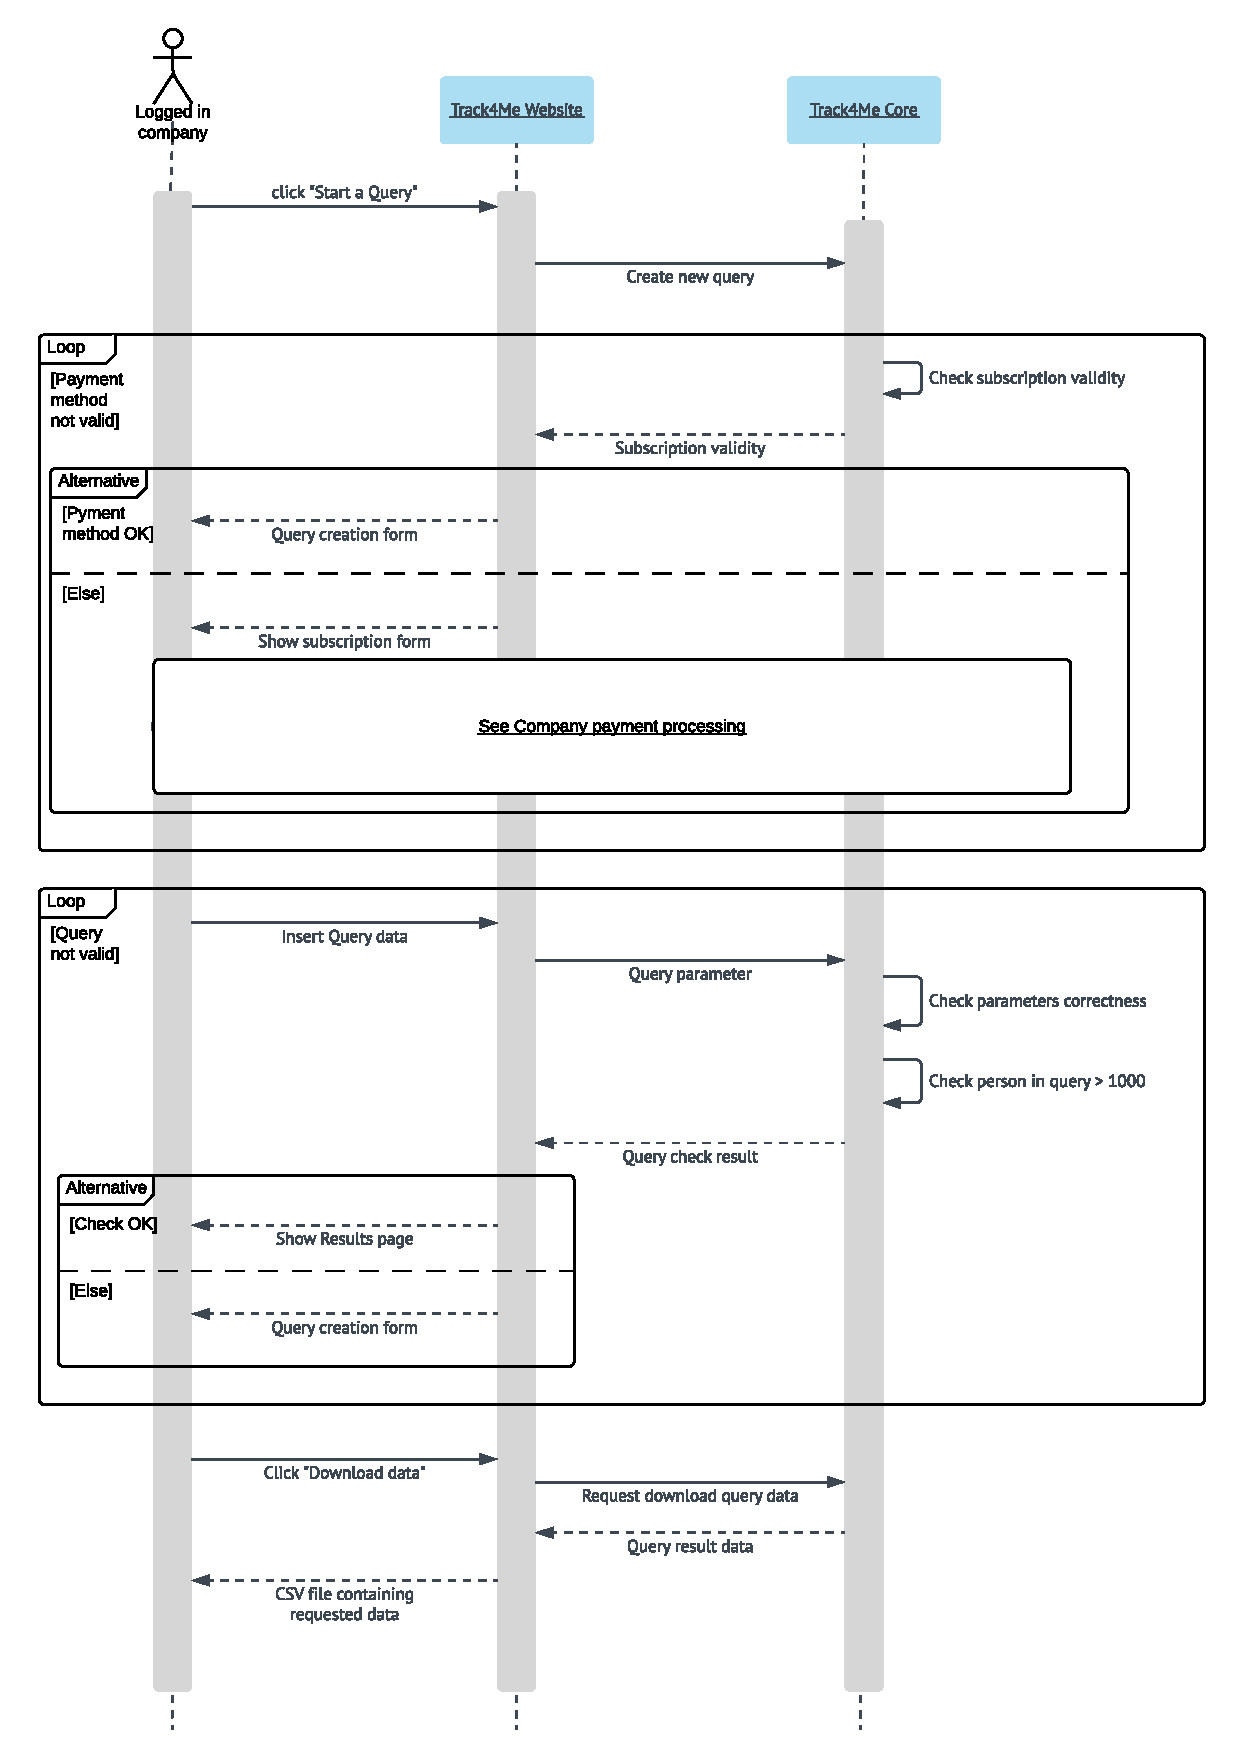
\includegraphics[width=\textwidth,height=\textheight,keepaspectratio]{assets/sequence/CompanyQuerySearchOnMultipleIndividuals.pdf}
  \caption{Company query search on multiple individuals sequence diagram}
  \label{fig:CompanyQuerySearchOnMultipleIndividuals}
\end{figure}
















\newpage
\paragraph{Company request for individual monitoring}
\begin{center}
\begin{table}[H]
\centering
\begin{tabular}{l|p{0.7\textwidth}}
\textbf{Actors} & Company, User, Core component \\
\textbf{Start conditions} & None \\
\textbf{Event flow}  & 

\begin{minipage}[t]{0.7\textwidth}
    \begin{itemize}
        \item Company clicks on add new patient 
\item System checks if the company can add new patients 
\item Company insert the username of the patient 
\item System checks if username exists in the database
\item System send a monitoring request notification to the user 
\item Username clicks on “Accept requests” through the Mobile app notification or through the email notification 
    \end{itemize}
    
\end{minipage}

\\
\textbf{Exit condition} & 
\begin{minipage}[t]{0.7\textwidth}
    \begin{itemize}
       \item System adds information of the monitoring company to the user in the database
\item The system update number of patient left to monitor of the company in the database

    \end{itemize}
    
\end{minipage}
\\
\textbf{Exceptions} & 

\begin{minipage}[t]{0.7\textwidth}
    \begin{itemize}
       \item No new patients left for the company type of subscription
\item Username not found
\item User refuses the request

    \end{itemize}
    
\end{minipage}
\\
\textbf{Goals} & G5 
\end{tabular}

\end{table}
\end{center}

\begin{figure}[H]
  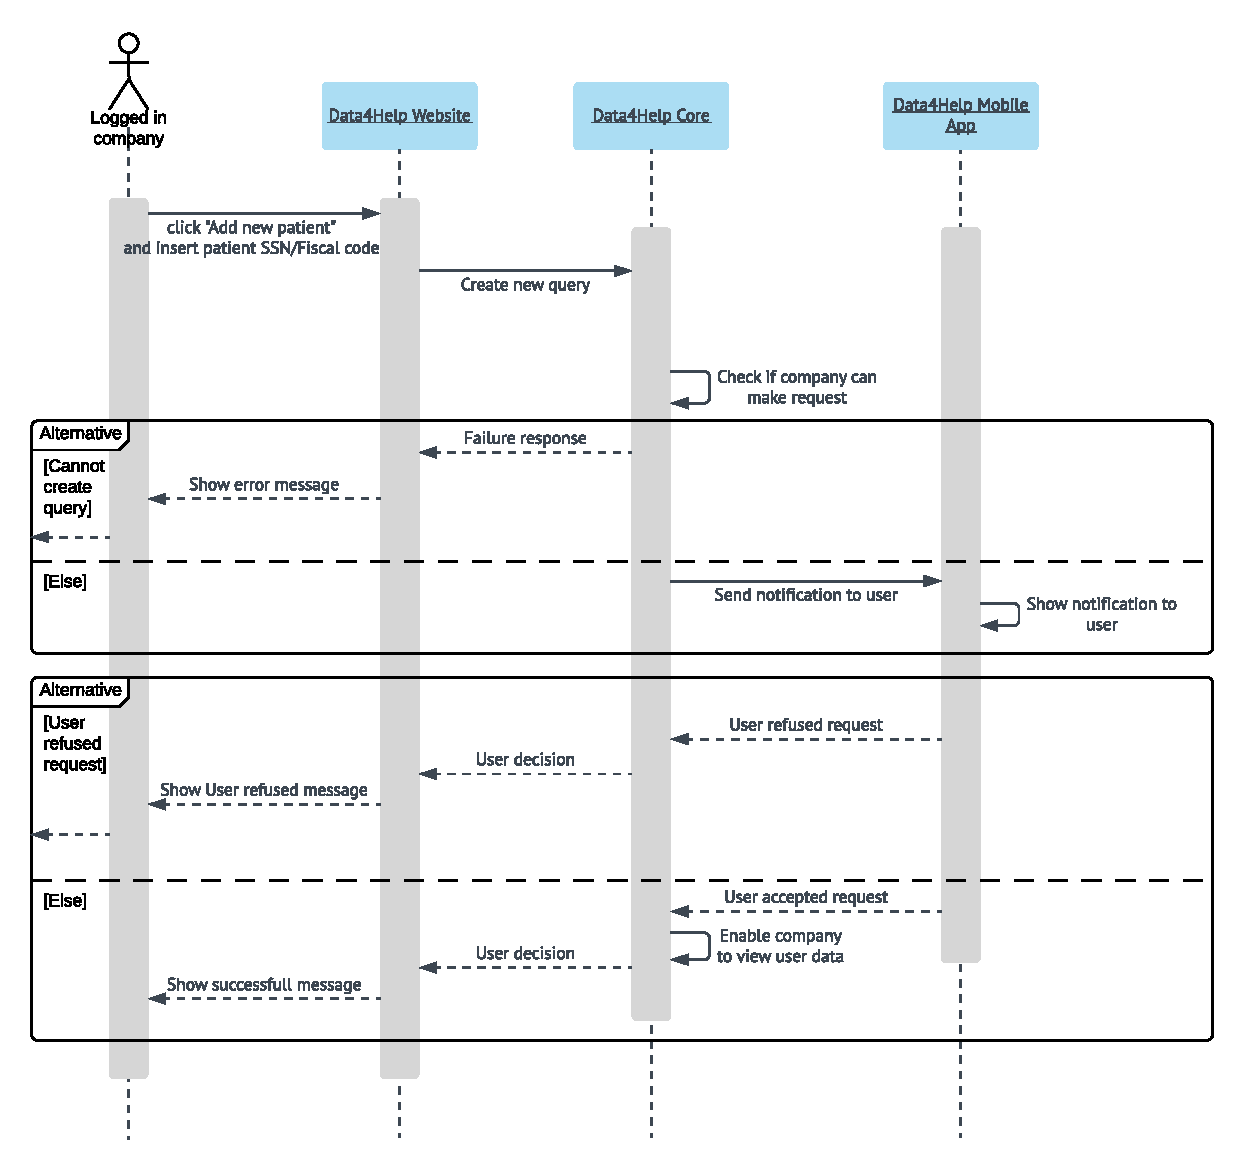
\includegraphics[width=\textwidth,height=\textheight,keepaspectratio]{assets/sequence/CompanyRequestForIndividualMonitoring.pdf}
  \caption{Company request for individual monitoring sequence diagram}
  \label{fig:CompanyRequestForIndividualMonitoring}
\end{figure}
















\newpage
\paragraph{Company consulting of individual data}
\begin{center}
\begin{table}[H]
\centering
\begin{tabular}{l|p{0.7\textwidth}}
\textbf{Actors} & Company, core component \\
\textbf{Start conditions} & None \\
\textbf{Event flow}  & 
\begin{minipage}[t]{0.7\textwidth}
    \begin{itemize}
        \item Company clicks on “See patients information” on the website

\item System shows a page listing all active patients for the company

\item Company clicks on the desired patient name

\item System shows all information of the patient and a menu where to choose a day 

\item Company chooses a day of the calendar from the menu
\item System shows the data of the patient on the specified day

    \end{itemize}
    
\end{minipage}\\
\textbf{Exit condition} & None \\
\textbf{Exceptions} & \begin{minipage}[t]{0.7\textwidth}
    \begin{itemize}
       \item No query left for the company type of subscription
        \item Not valid query

    \end{itemize}
    
\end{minipage} \\
\textbf{Goals} & G5 
\end{tabular}

\end{table}
\end{center}
\begin{figure}[H]
  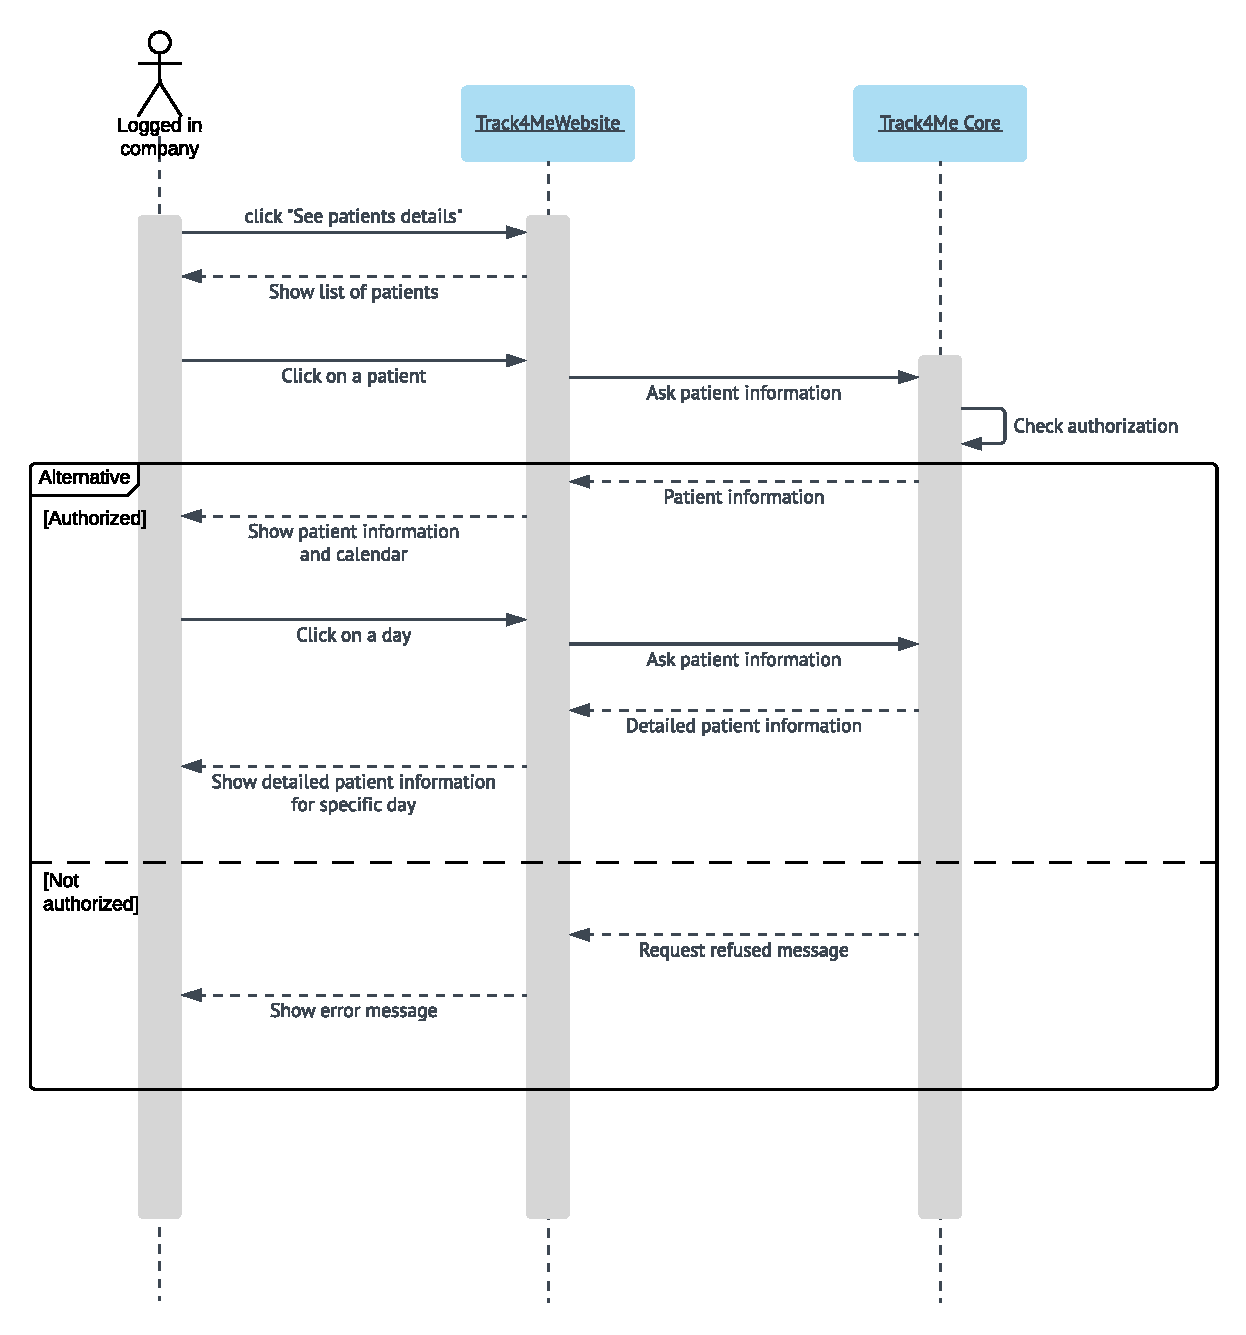
\includegraphics[width=\textwidth,height=\textheight,keepaspectratio]{assets/sequence/CompanyConsultingOfIndividualData.pdf}
  \caption{Company consulting of individual data sequence diagram}
  \label{fig:CompanyConsultingOfIndividualData}
\end{figure}













\newpage
\paragraph{Company payment processing}
\begin{center}
\begin{table}[H]
\centering
\begin{tabular}{l|p{0.7\textwidth}}
\textbf{Actors} & Company, Core component \\
\textbf{Start conditions} & Company purchases a subscription plan \\
\textbf{Event flow}  & \begin{minipage}[t]{0.7\textwidth}
    \begin{itemize}
       \item Company insert the number of the credit card and the CVV
\item System verify the card has enough money
\item The system get the money from the credit card
\item The system show a Successful operation 


    \end{itemize}
    
\end{minipage} \\
\textbf{Exit condition} & The system stored the information of the subscription of the company in the database \\
\textbf{Exceptions} & \begin{minipage}[t]{0.7\textwidth}
    \begin{itemize}
       \item Not enough money
        \item Not valid credit card information
    \end{itemize}
    
\end{minipage} \\
\textbf{Goals} & G6 
\end{tabular}

\end{table}
\end{center}


\begin{figure}[H]
  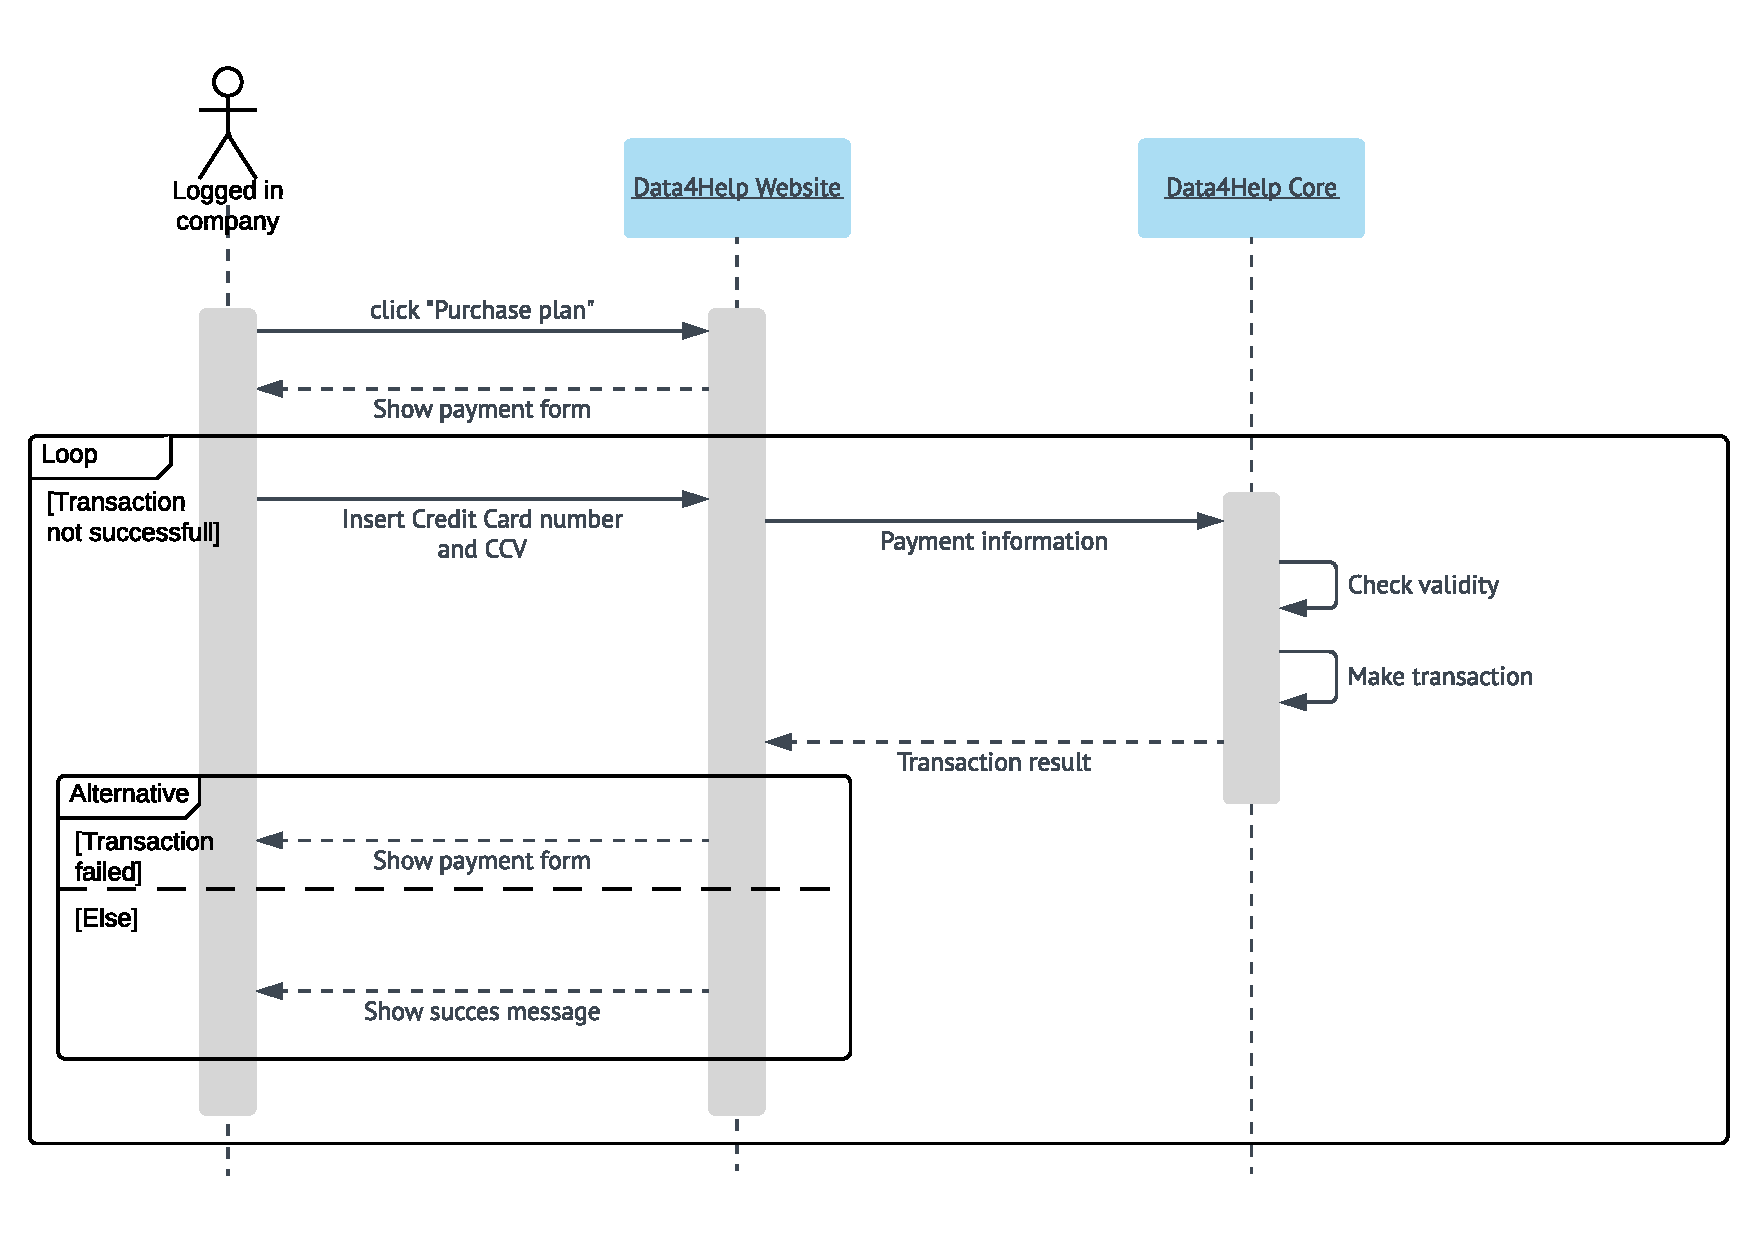
\includegraphics[width=\textwidth,height=\textheight,keepaspectratio]{assets/sequence/CompanyPaymentProcessing.pdf}
  \caption{Company payment processing sequence diagram}
  \label{fig:CompanyPaymentProcessing}
\end{figure}











\newpage
\paragraph{Company receives data of subscribed query}
\begin{center}
\begin{table}[H]
\centering
\begin{tabular}{l|p{0.7\textwidth}}
\textbf{Actors} & 
Company, core component
 \\
\textbf{Start conditions} & Is 0:01 of one month passed after the last data sent of the query \\
\textbf{Event flow}  & \begin{minipage}[t]{0.7\textwidth}
    \begin{itemize}
       \item System retrieve the query information on the database

        \item System compute query on the database
        \item System export a CSV of the data stored
        \item System send the document on the email of the company 


    \end{itemize}
    
\end{minipage} \\
\textbf{Exit condition} & None \\
\textbf{Exceptions} & None \\
\textbf{Goals} & \textbf{G7} 
\end{tabular}

\end{table}
\end{center}

\begin{figure}[H]
  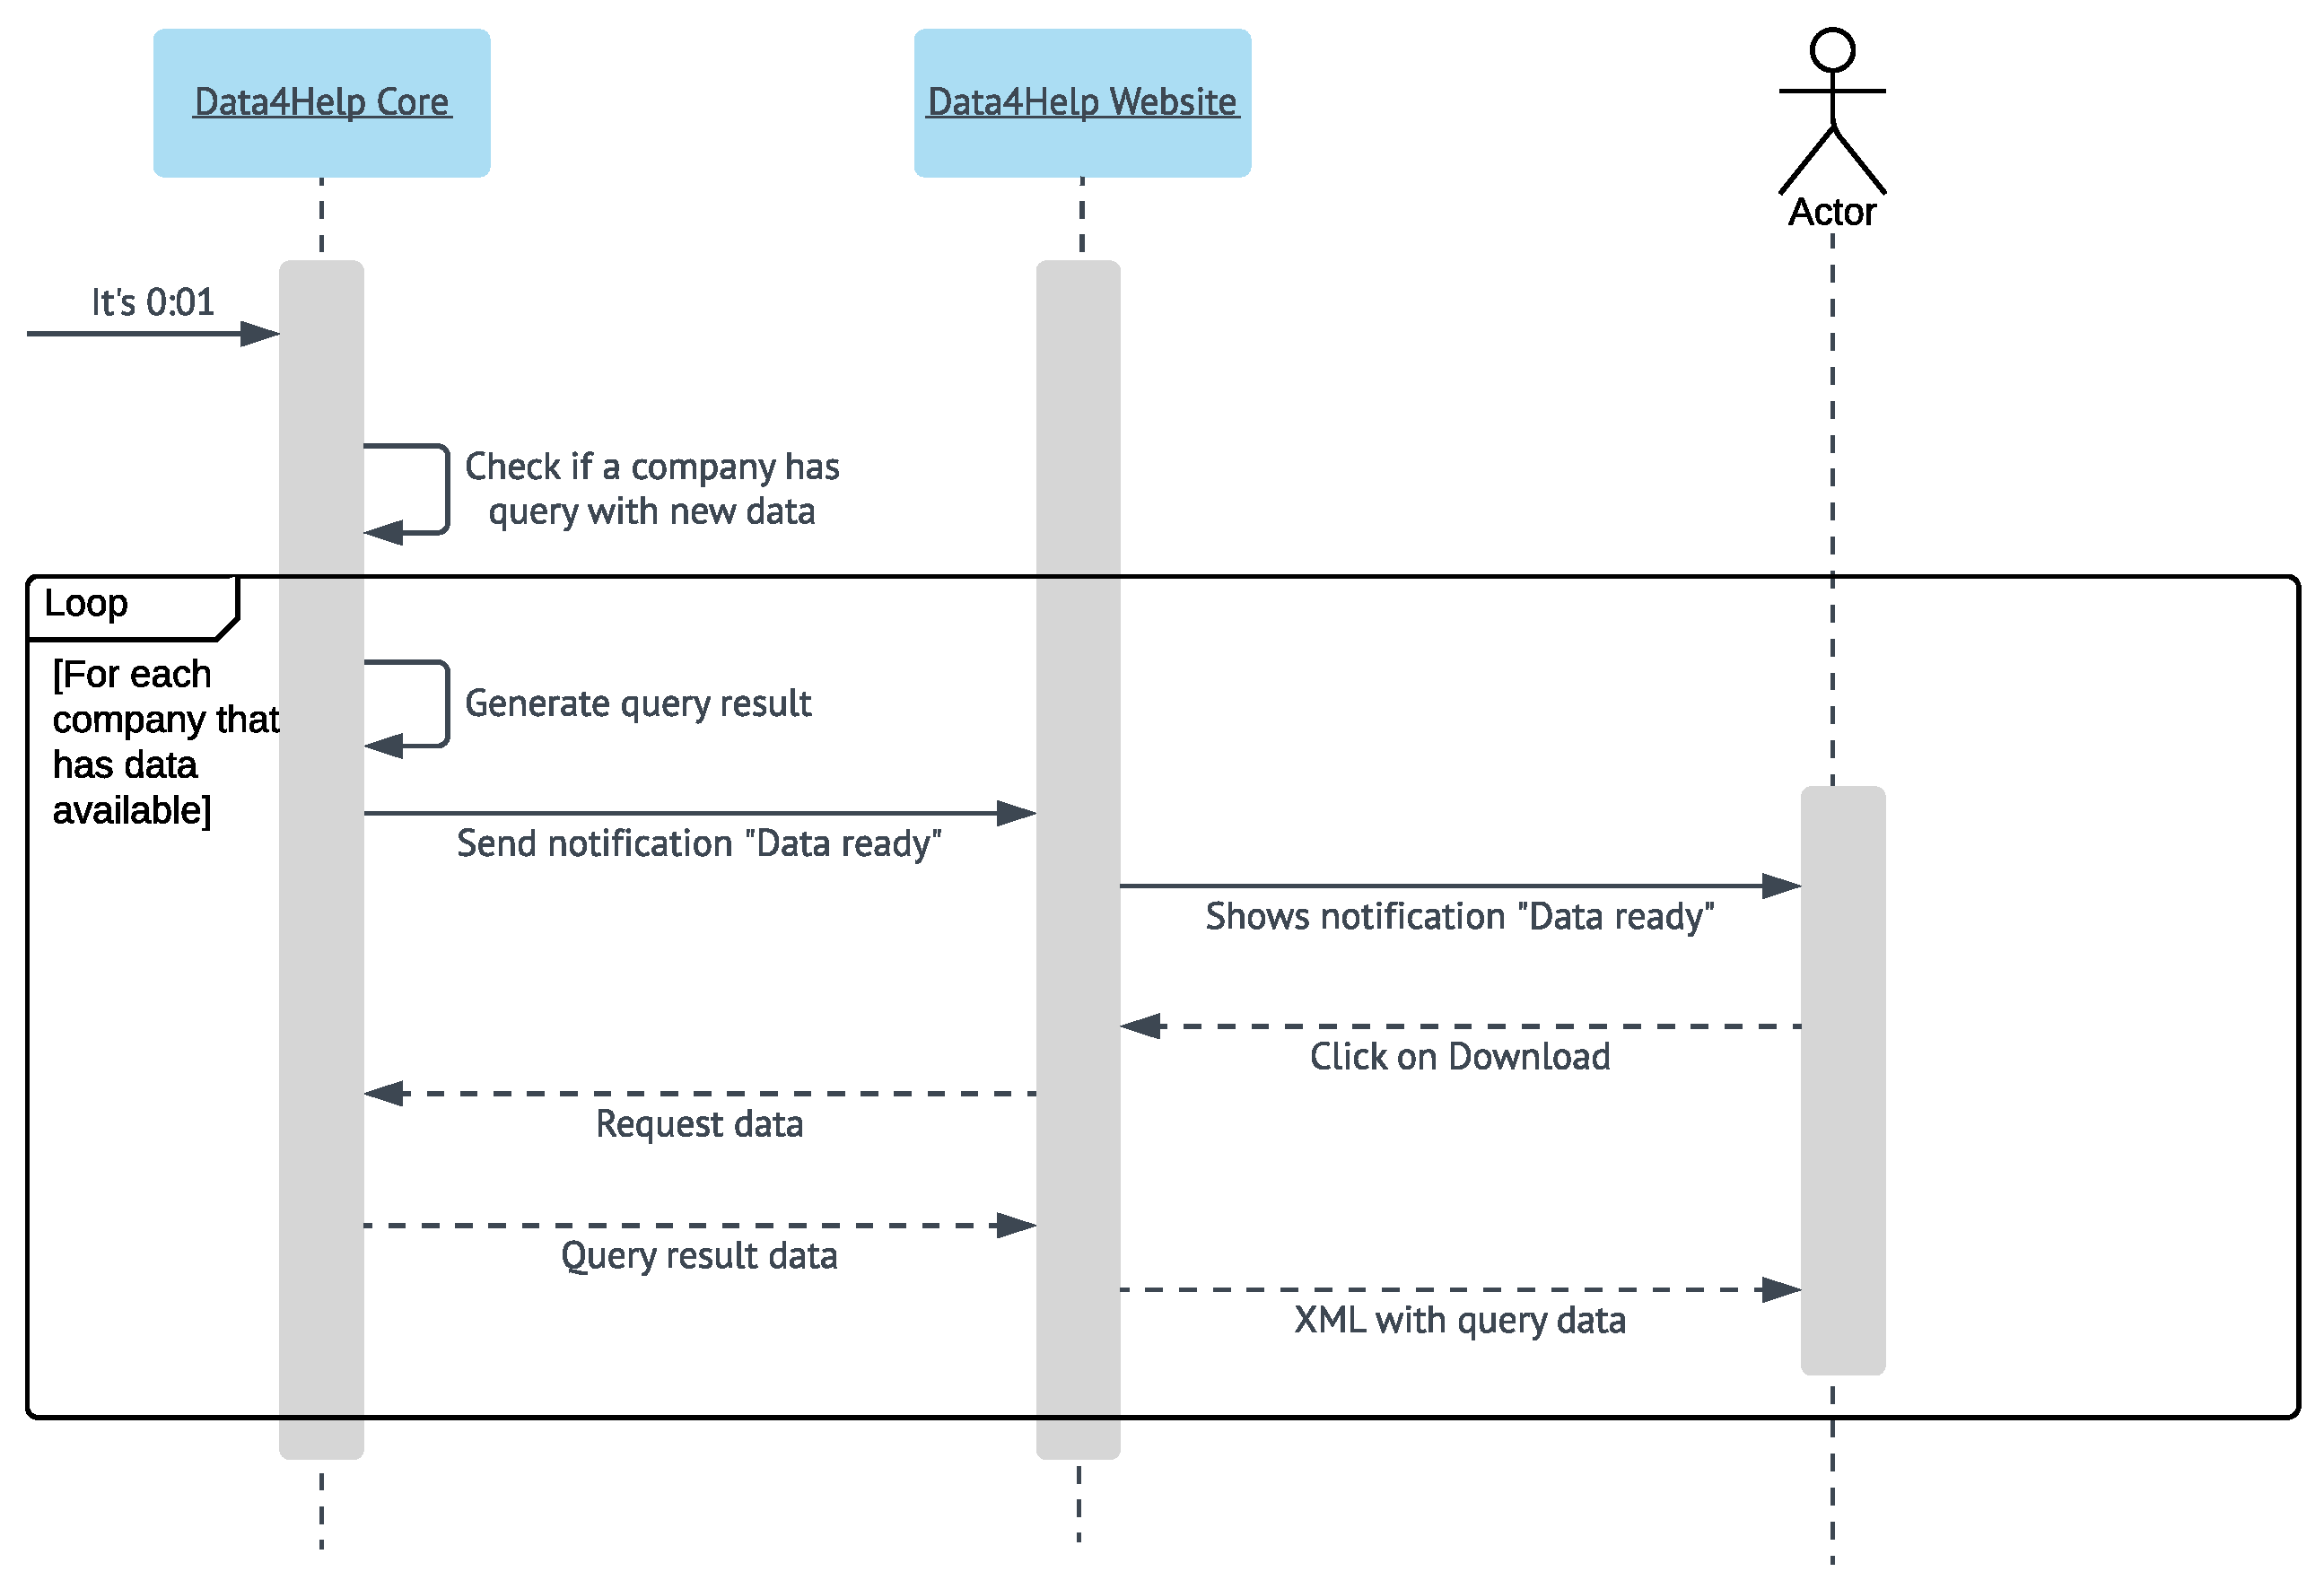
\includegraphics[width=\textwidth,height=\textheight,keepaspectratio]{assets/sequence/CompanyReceivesDataOfSubscribedQuery.pdf}
  \caption{Company receives data of subscribed query sequence diagram}
  \label{fig:CompanyReceivesDataOfSubscribedQuery}
\end{figure}

















\newpage
\paragraph{Emergency situation and ambulance call}
\begin{center}
\begin{table}[H]
\centering
\begin{tabular}{l|p{0.7\textwidth}}
\textbf{Actors} & User, core component \\
\textbf{Start conditions} & User health parameter under the threshold value \\
\textbf{Event flow}  & \begin{minipage}[t]{0.7\textwidth}
    \begin{itemize}
       \item System change the user status in “AMBULANCE NEED”
\item System connects hospital API 
\item Hospital API answer to the connection
\item System send emergency request to the hospital API sending location of the user and the health parameters under the threshold
\item Hospital API confirms that an ambulance has been sent to the position

    \end{itemize}
    
\end{minipage} \\
\textbf{Exit condition} & The user is labelled as “AMBULANCE SENT” \\
\textbf{Exceptions} & Hospital API refuses the connection \\
\textbf{Goals} & G9 
\end{tabular}

\end{table}
\end{center}
\begin{figure}[H]
  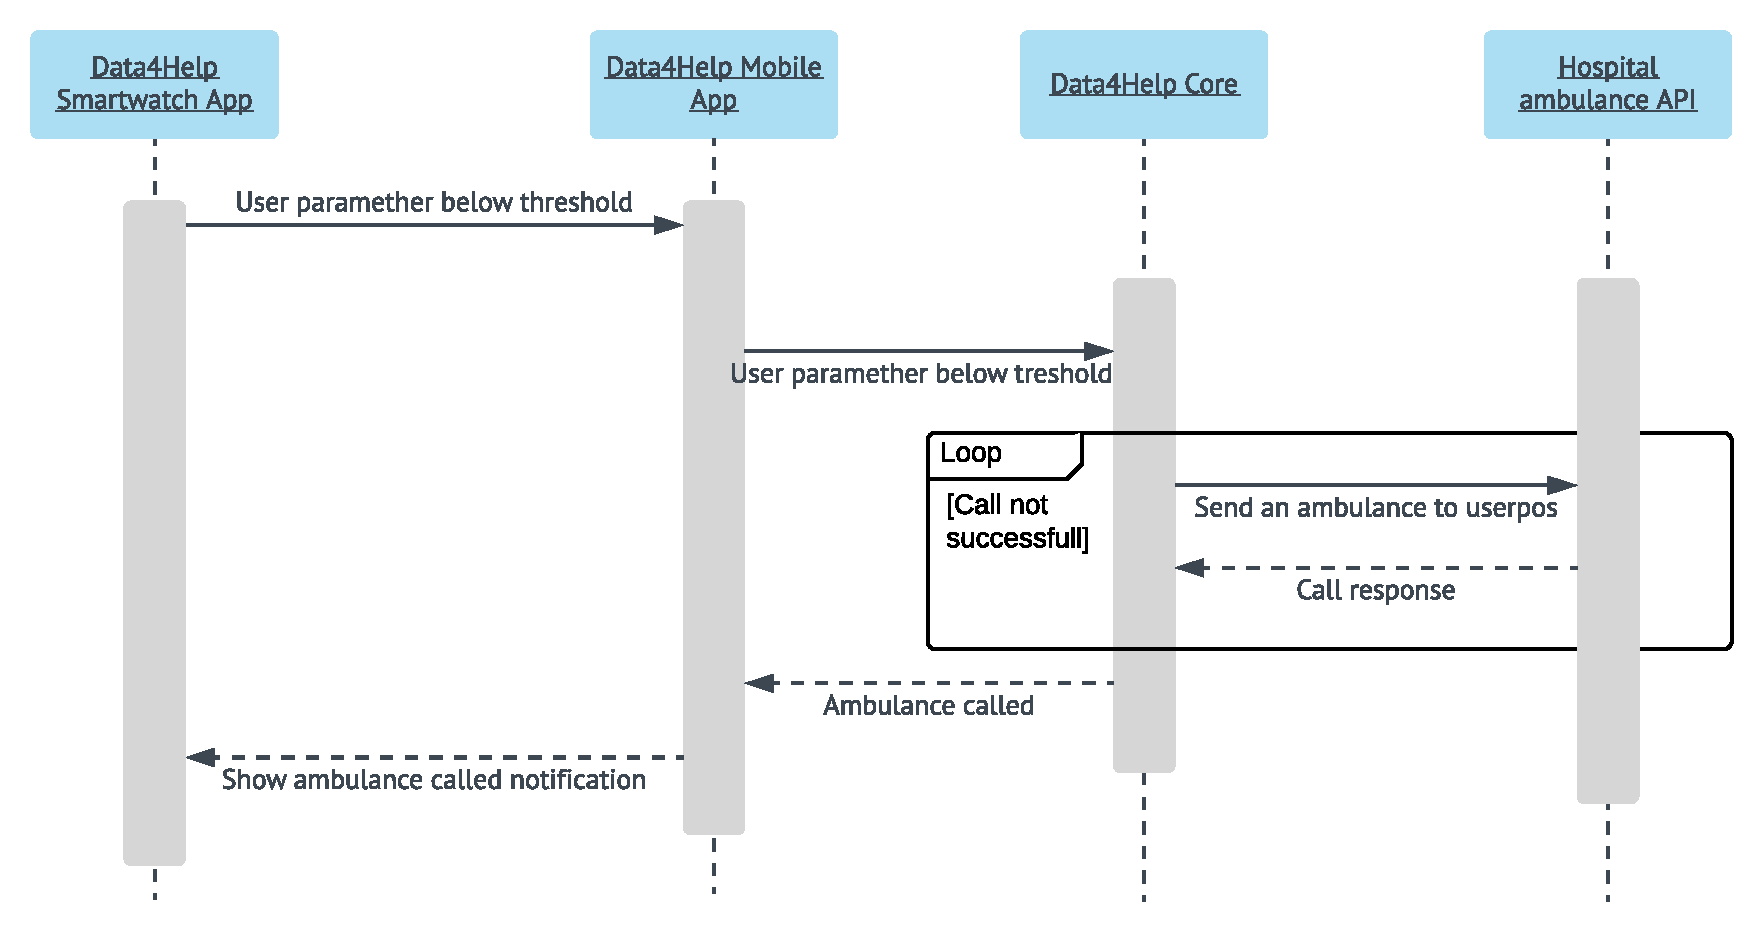
\includegraphics[width=\textwidth,height=\textheight,keepaspectratio]{assets/sequence/EmergencySituationAndAmbulanceCall.pdf}
  \caption{Emergency situation and ambulance call sequence diagram}
  \label{fig:EmergencySituationAndAmbulanceCall}
\end{figure}












\newpage
\paragraph{Run organizer registration}
\begin{center}
\begin{table}[H]
\centering
\begin{tabular}{l|p{0.7\textwidth}}
\textbf{Actors} & Not registered run organizer \\
\textbf{Start conditions} & None \\
\textbf{Event flow}  & \begin{minipage}[t]{0.7\textwidth}
    \begin{itemize}
       \item not registered company run organizer clicks on “Subscribe”
\item not registered run organizer inserts a username, an email and a password
\item The system checks if email is not used by any other user
\item The system generates a confirmation mail
\item The run organizer confirms the registration click on “Confirm email”
\item The system shows a registration complete screen


    \end{itemize}
    
\end{minipage} \\
\textbf{Exit condition} & Run organizer information used for registering is stored in the Data4Help database \\
\textbf{Exceptions} & \begin{minipage}[t]{0.7\textwidth}
    \begin{itemize}
       \item Not valid username
\item Not valid email
    \end{itemize}
    
\end{minipage} \\ \\
\textbf{Goals} & G10
\end{tabular}

\end{table}
\end{center}
\begin{figure}[H]
  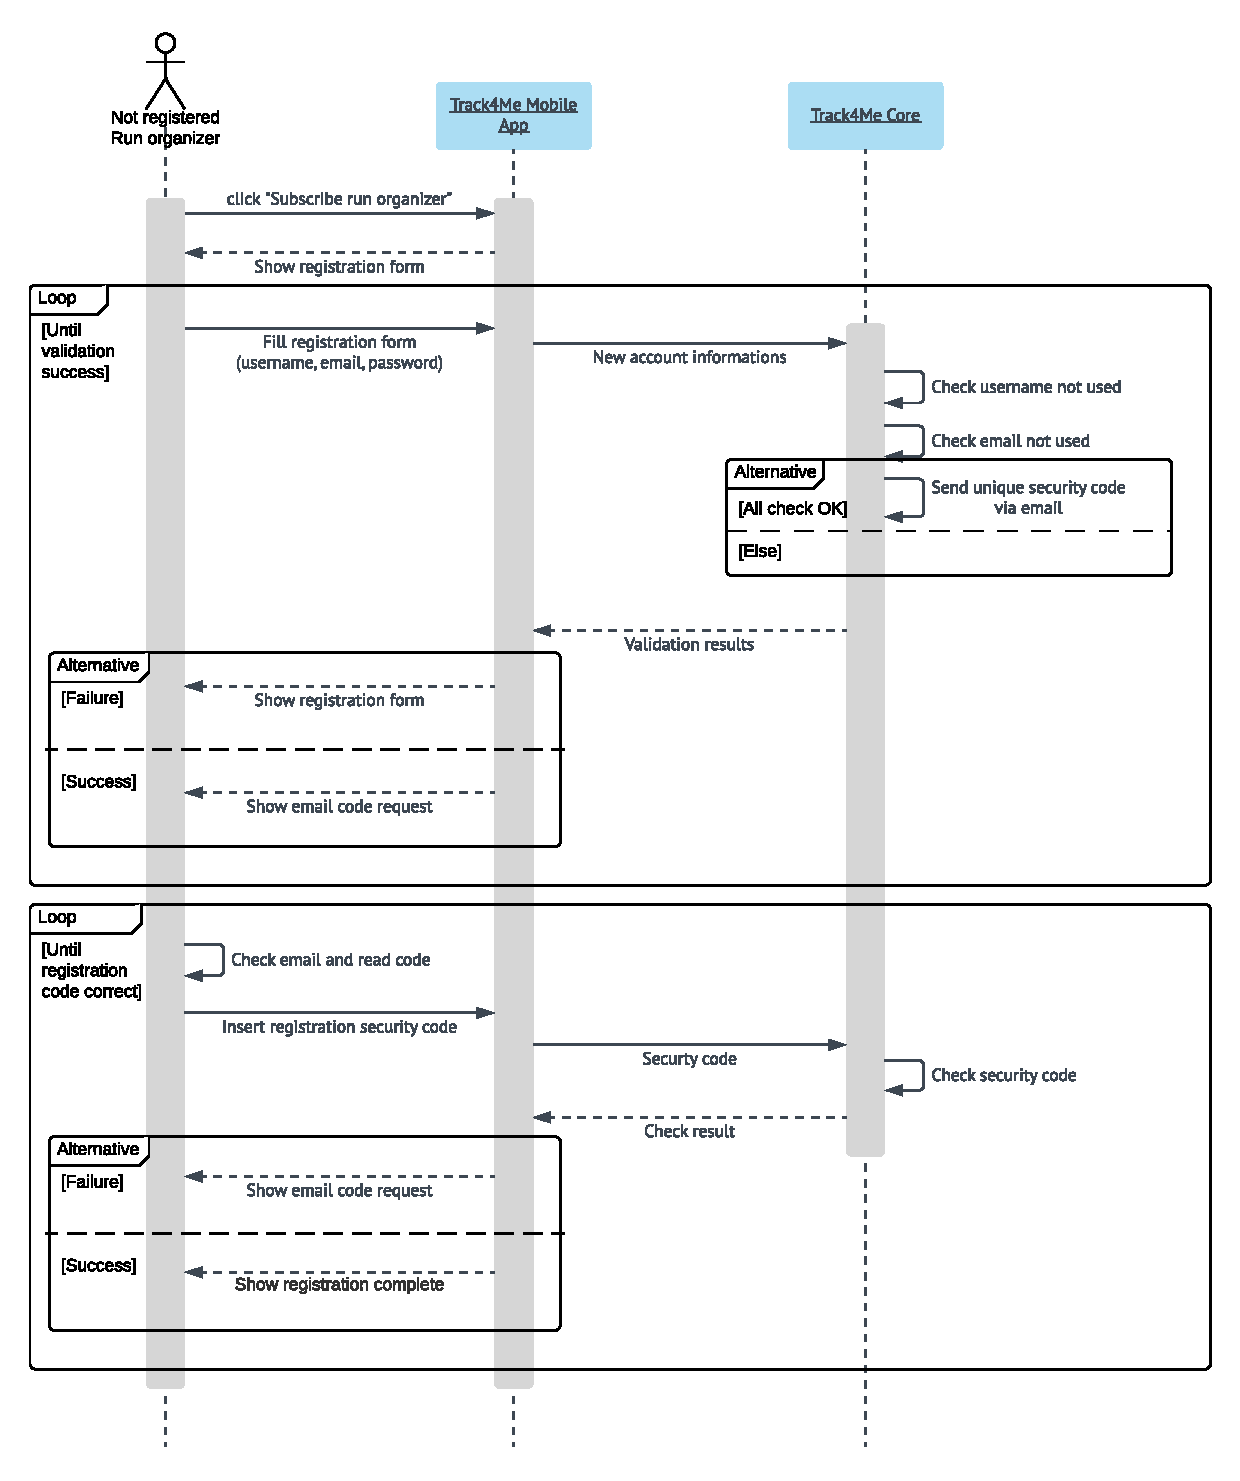
\includegraphics[width=\textwidth,height=\textheight,keepaspectratio]{assets/sequence/RunOrganizerRegistration.pdf}
  \caption{Run organizer registration sequence diagram}
  \label{fig:RunOrganizerRegistration}
\end{figure}















\newpage
\paragraph{Run organizer adds a new race}
\begin{center}
\begin{table}[H]
\centering
\begin{tabular}{l|p{0.7\textwidth}}
\textbf{Actors} & Run organizer \\
\textbf{Start conditions} & None \\
\textbf{Event flow}  & \begin{minipage}[t]{0.7\textwidth}
    \begin{itemize}
    \item Run organizer clicks on "Organize new run" on the Data4Help website 
    \item The system shows a screen with empty spaces about run information
    \item Run organizer insert the name of the run, the city where the run will take place, the date and the starting time
    \item The system checks if date is correct
    \item The system shows a map where user can define the path of the run
    \item Run organizer clicks on the path he wants the run to be taken
    \item The system calculates the km of the run
    \item The system show a "Correctly created run" screen
\end{itemize}
    
\end{minipage} \\
\textbf{Exit condition} & The system stores the information of the run in the Data4Help database and makes it public to users \\
\textbf{Exceptions} & \begin{minipage}[t]{0.7\textwidth}
    \begin{itemize}
\item Not valid date
    \end{itemize}
    
\end{minipage} \\ \\
\textbf{Goals} & G11
\end{tabular}

\end{table}
\end{center}

\begin{figure}[H]
  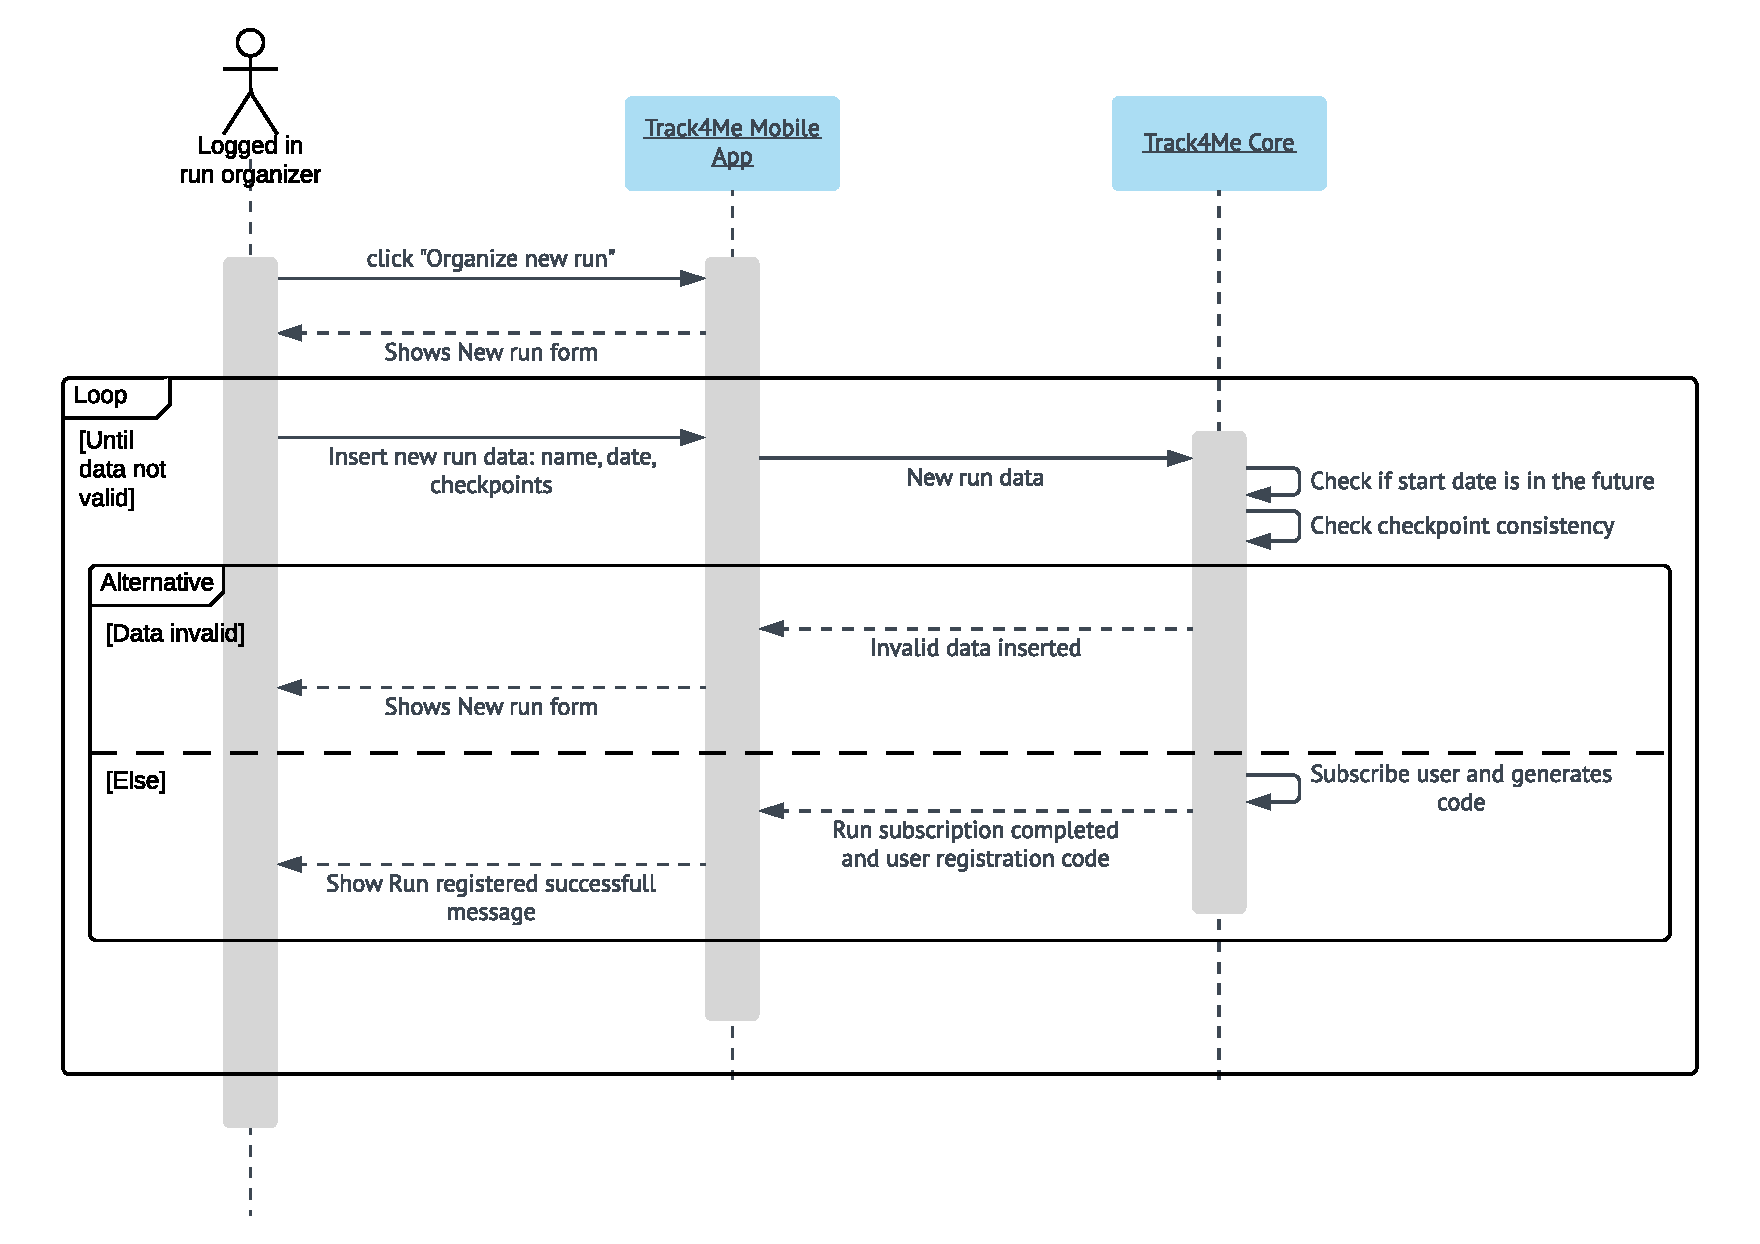
\includegraphics[width=\textwidth,height=\textheight,keepaspectratio]{assets/sequence/RunOrganizerAddsANewRace.pdf}
  \caption{Run organizer adds a new race sequence diagram}
  \label{fig:RunOrganizerAddsANewRace}
\end{figure}









\newpage
\paragraph{Runner subscription to a race}
\begin{center}
\begin{table}[H]
\centering
\begin{tabular}{l|p{0.7\textwidth}}
\textbf{Actors} & Run organizer\\
\textbf{Start conditions} & None \\
\textbf{Event flow}  & \begin{minipage}[t]{0.7\textwidth}
    \begin{itemize}
       \item Partecipant clicks on 'See nearby races'

        \item System shows a map with the races closer than 2 km from the user

\item Partecipant click on a run and clicks subscribe
\item The system verifies if it's still possible to subscribe

\item The system generates an runner ID number for the user
\item The system send the ID number to the user email
\item The user shows a correct subscription screenshot on the Mobile app

    \end{itemize}
    \end{minipage}
    \\
\textbf{Goals} & G12
\end{tabular}

\end{table}
\end{center}

\begin{figure}[H]
  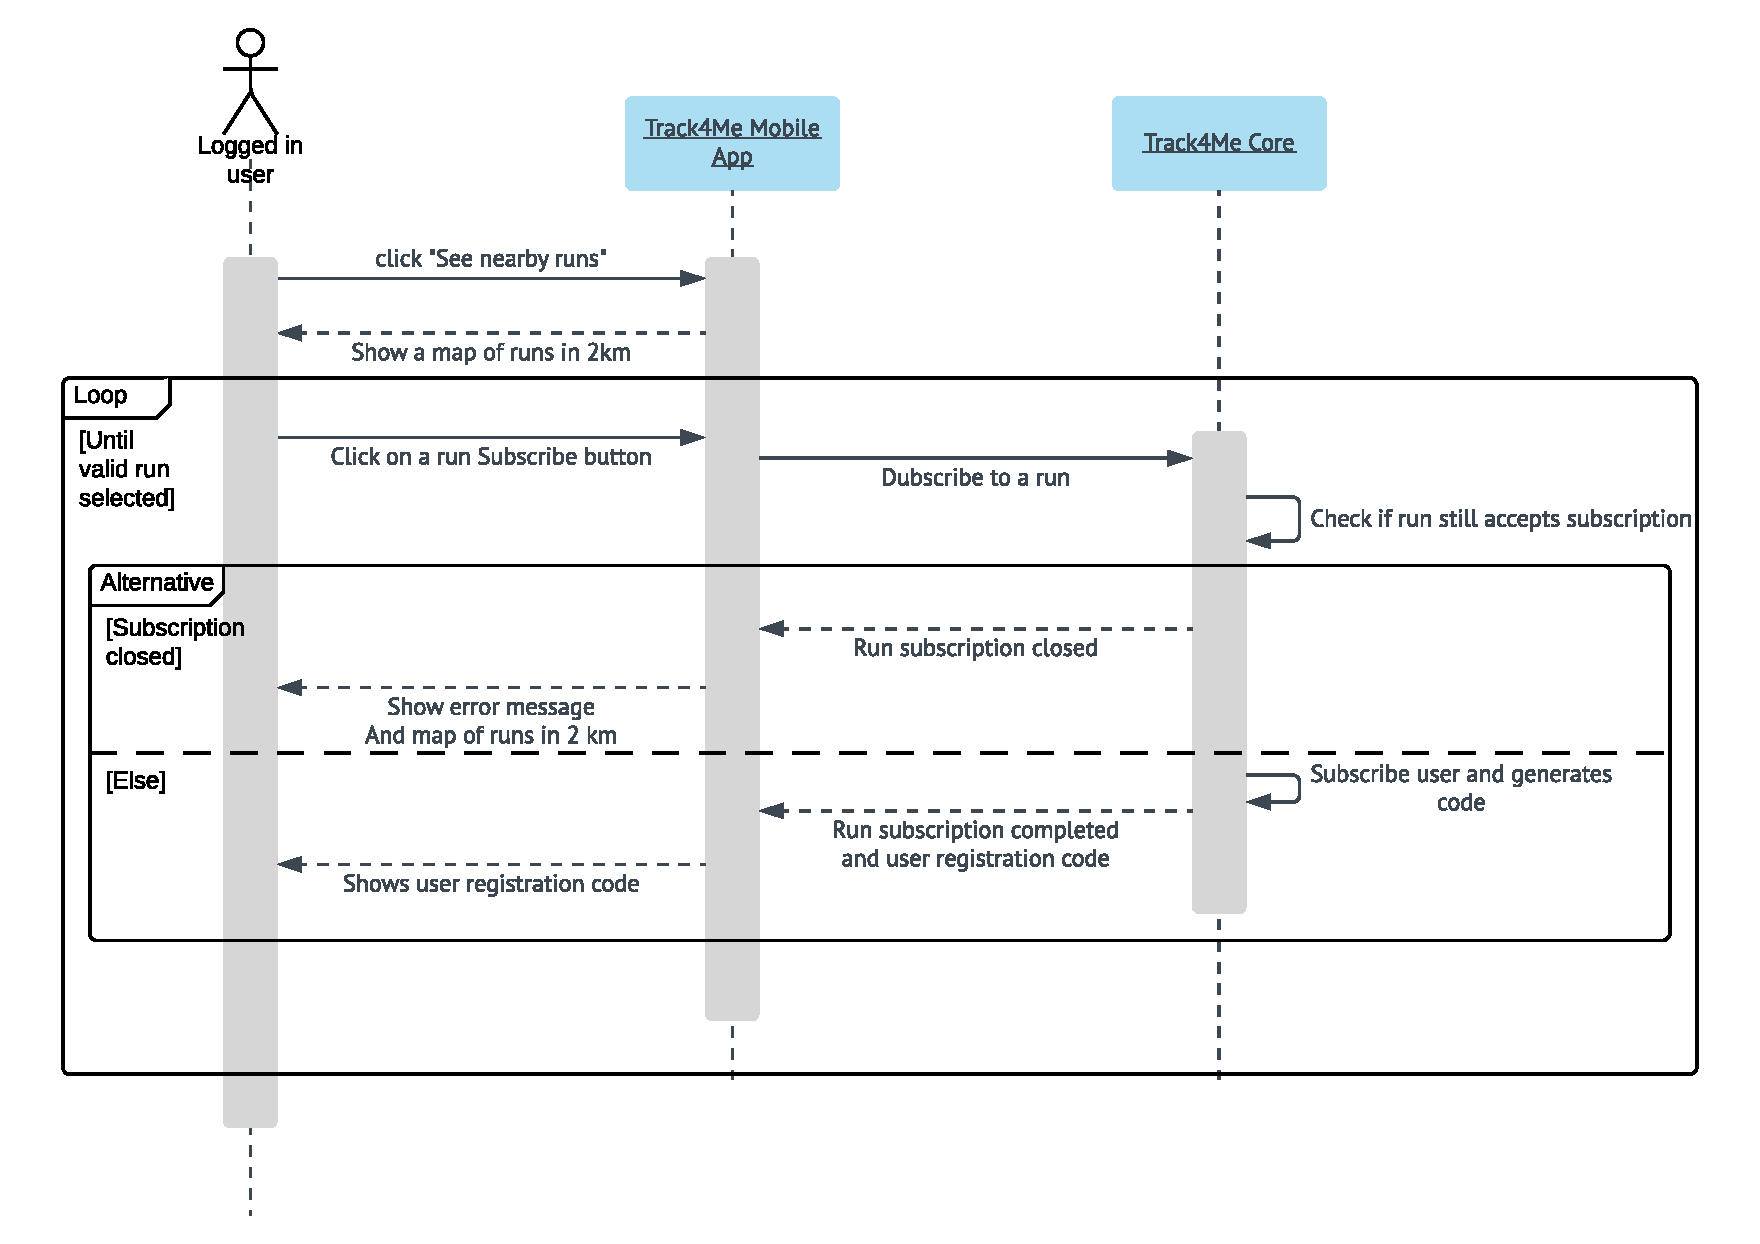
\includegraphics[width=\textwidth,height=\textheight,keepaspectratio]{assets/sequence/RunnerSubscriptionToARace.pdf}
  \caption{Runner subscription to a race sequence diagram}
  \label{fig:RunnerSubscriptionToARace}
\end{figure}







\newpage
\paragraph{Spectator or a run requests for runner position}
\begin{center}
\begin{table}[H]
\centering
\begin{tabular}{l|p{0.7\textwidth}}
\textbf{Actors} & User \\
\textbf{Start conditions} & None \\
\textbf{Event flow}  & \begin{minipage}[t]{0.7\textwidth}
    \begin{itemize}
       \item User clicks on "See nearby races"
\item System shows the map in radius of 2km from the user current position
\item User clicks on the desired run he wants to see and clicks on “see current runner positions”
\item The system shows a map with runners geographical position with their relative username and rank


    \end{itemize}
    
\end{minipage}  \\
\textbf{Exit condition} & None \\
\textbf{Exceptions} & \begin{minipage}[t]{0.7\textwidth}
    \begin{itemize}
       \item Run has already finished
\item Run hasn't already started


    \end{itemize}
    
\end{minipage}  \\
\textbf{Goals} & G13 
\end{tabular}

\end{table}
\end{center}

\begin{figure}[H]
  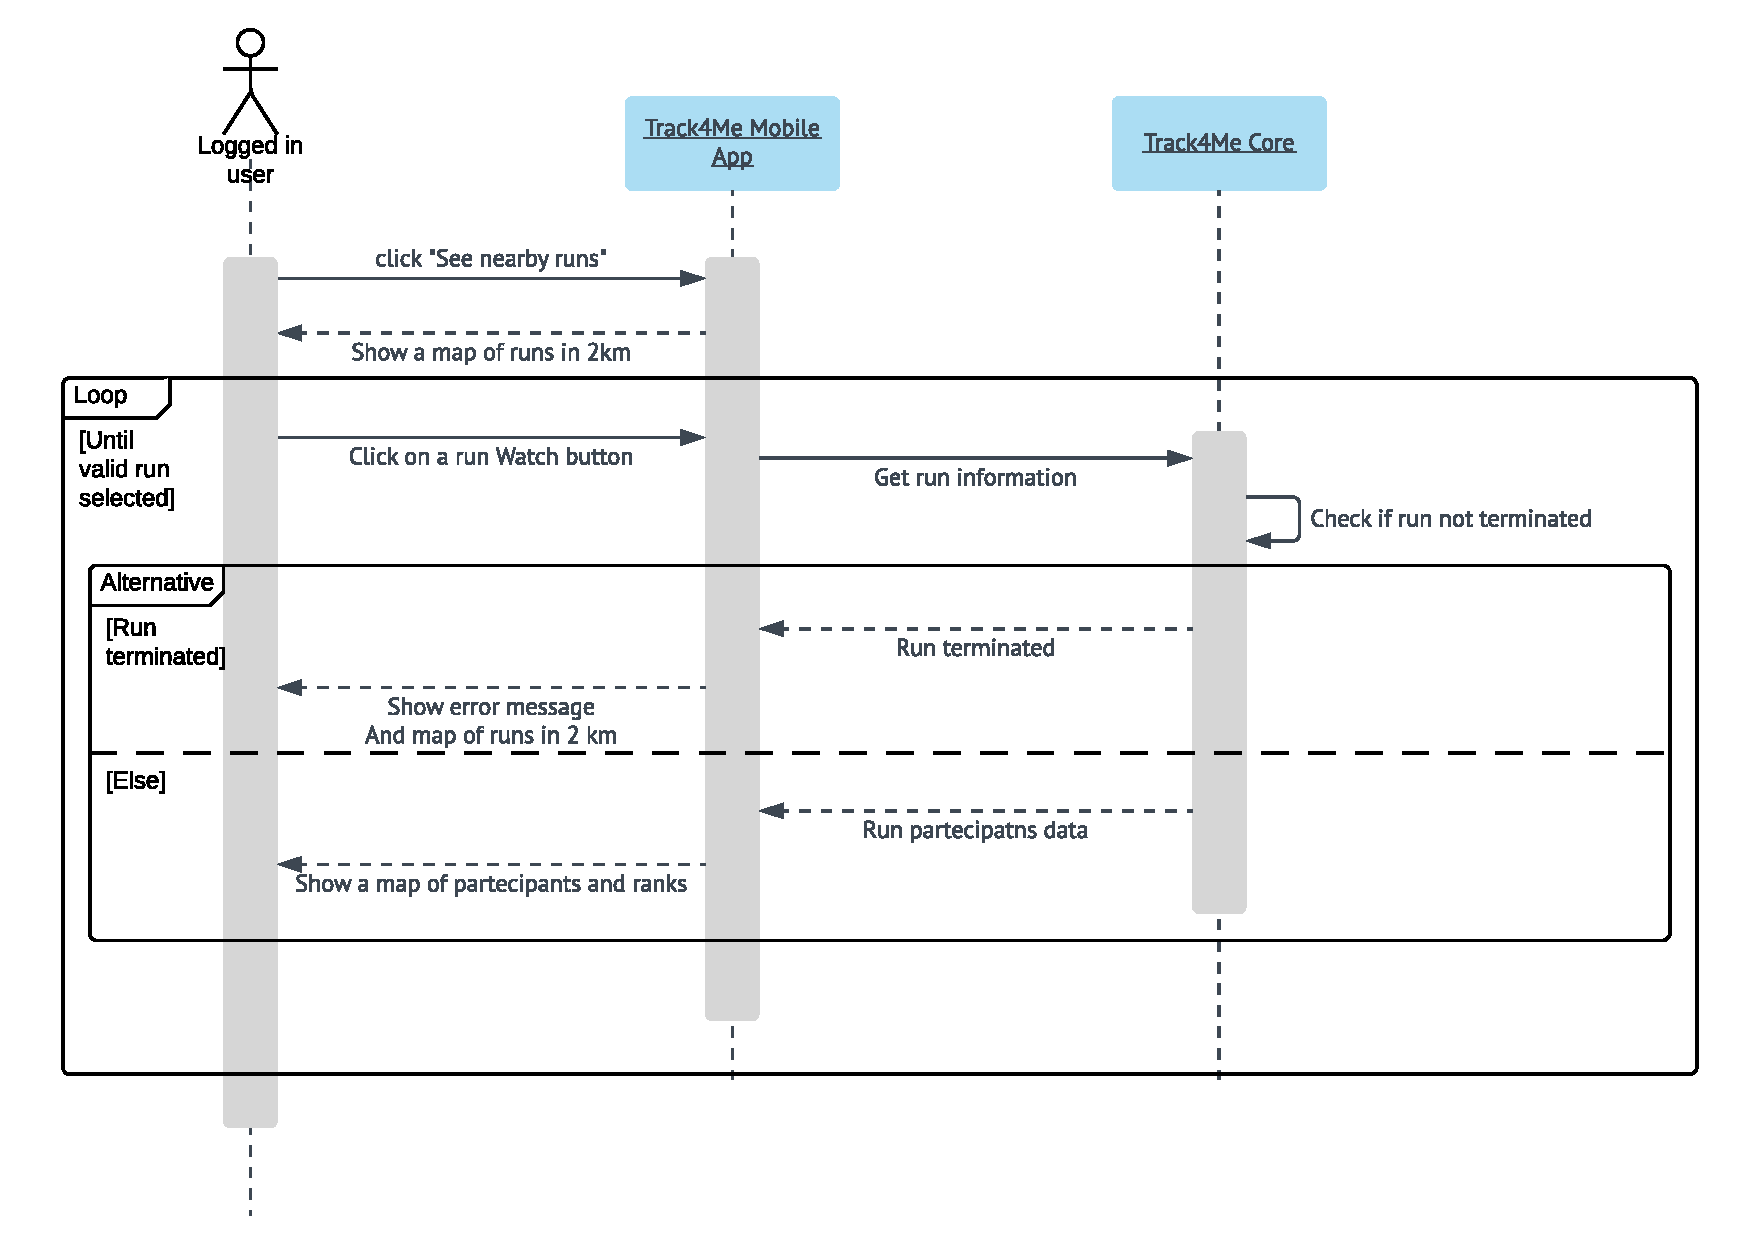
\includegraphics[width=\textwidth,height=\textheight,keepaspectratio]{assets/sequence/SpectatorOfARunRequestsForRunnerPosition.pdf}
  \caption{Spectator or a run requests for runner position sequence diagram}
  \label{fig:SpectatorOfARunRequestsForRunnerPosition}
\end{figure}


        \section{Appendix}
            \subsection{Alloy}
                \begin{verbatim}
    open util/boolean

// Signatures

sig CharSet {}

sig Position {
    _lat: one CharSet,
    _long: one CharSet
}

sig Smartwatch {
    user: one User,
    compatible: one Bool
}

abstract sig Customer {
    username: lone CharSet, 
    password: lone CharSet,
    canRegister: one Bool,
    isRegistered: one Bool
} {
    isRegistered = True => canRegister = True
    canRegister = False => isRegistered = False
    (#username = 0 || #password = 0) => isRegistered = False 
}

sig User extends Customer {
    fiscalCodeOrSSN: lone CharSet,
    smartwatch: one Smartwatch,
    notifications: set Notification, 
    acceptsDataRequestFrom: set Company,
    hasInscriptionCode: lone Bool,
} {
    (
        #fiscalCodeOrSSN = 0 || 
        smartwatch.compatible = False
    ) <=> (canRegister = False)
}

sig Elderly extends User {
    isInDanger: one Bool,
    inDangerFrom: lone Int
} {
    inDangerFrom >= 0 => isInDanger = True
    #inDangerFrom = 0 => isInDanger = False
}

sig AmbulanceRequest {
    hospital: one Company,
    person: one Elderly,
    timeElapsed: one Int,
    accepted: one Bool
} {
    timeElapsed >= 5 => accepted = True
}
sig RunOrganizer extends User {
    runPath: set Position,
    runOrganized: lone Run
} {
    isRegistered = False => (#runPath = 0 && #runOrganized = 0)
}

sig Company extends Customer {
    paymentMethod: lone CharSet,
    queries: set Query
} {
    #paymentMethod = 0 <=> canRegister = False
    isRegistered = False => #queries = 0
}

abstract sig Query {
    company: one Company
}

sig AnonQuery extends Query {
    people: set User,
    isValid: one Bool
} {
    isValid = True <=> #people >= 3
    no p: User | p in people && p.isRegistered = False
}

sig IndividualQuery extends Query {
    person: one User,
    userAccepts: lone Bool, 
} 

sig Notification {
    user: one User,
    company: one Company
}

sig Run {
    hasStarted: one Bool,
    participants: set User,
    organizer: one RunOrganizer
}

// Facts: Consistency

fact UsernameConsistency {
    // There are no 2 Customer(s) with the same username
    all disj c, c': Customer | c.username != c'.username
}

fact FiscalCodeOrSSNConsistency {
    // There are no 2 User(s) with the same fiscalCodeOrSSN
    all disj u, u': User | u.fiscalCodeOrSSN != u'.fiscalCodeOrSSN
}

fact SmartWatchConsistency {
    // Let's suppose, wlog, that the cardinality of the relation
    // between smartwatch and user is 1 to 1
    all s: Smartwatch, u: User | s.user = u <=> u.smartwatch = s
}

fact QueryConsistency {
    // If a query has been made by a company
    // it must be in the set of all the queries 
    // made by the company
    all q: Query, c: Company | q.company = c <=> q in c.queries
}

fact NotificationConsistency {
    // If a notification has been sent to a user
    // the user must have it in the set of 
    // all notifications
    all n: Notification, u: User | n.user = u <=> n in u.notifications
}

fact AmbulanceRequestConsistency {
    all e: Elderly, a: AmbulanceRequest | a.person = e <=> a.hospital in e.acceptsDataRequestFrom
}

fact RunAndRunOrganizerConsistency {
    all r: Run, ro: RunOrganizer {
        r.organizer = ro <=> ro.runOrganized = r
    }
}

// Assertions 

// Goal G2: The system should allow users to register.

assert UserCanRegister {
    all u: User {
        (
            #u.username = 1 && 
            #u.password = 1 && 
            #u.fiscalCodeOrSSN = 1 &&
            u.(smartwatch.compatible) = True
        ) => u.canRegister = True
    }
}

check UserCanRegister for 5

// Goal G3: The system should allow companies to register

assert CompaniesCanRegister {
    all c: Company {
        (
            #c.username = 1 && 
            #c.password = 1 &&  
            #c.paymentMethod = 1 
        ) => c.canRegister = True
    }
}
check CompaniesCanRegister for 5

// Goal G4: The system should allow registered companies to request data
// from an anonymized group of individuals, only if individuals in the
// group are more than 1000.

assert CompaniesCanMakeAnonimizedQueries {
    all c: Company, q: AnonQuery{
        (
            c.isRegistered = True && 
            #queries > 0 && 
            #q.people >= 5
        ) => q.isValid = True && q in c.queries

    }
}

check CompaniesCanMakeAnonimizedQueries for 5

// Goal G5: The system should allow registered companies to request data
// from an individual person, only if individuals accept the request.

assert CompaniesCanMakeIndividualQueries {
    
    // If a company requests data from a single person 
    // either
    // the person accepts <=> company is in the person acceptance list
    // or 
    // the person still hasn't accepted => there's a notification 
    // concerning the company and the user in the person notification list

    all q: IndividualQuery, c: Company, n: Notification {
        (q.company = c) &&
        (
            (q.userAccepts = True <=> c in q.(person.acceptsDataRequestFrom)) ||
            (#q.userAccepts = 0 => (
                n.user = q.person && 
                n.company = c && 
                n in q.(person.notifications)
            )) 
        )
    }
}

check CompaniesCanMakeAnonimizedQueries for 5

// Goal G11: If a run organizer is registered, it can define a run. For instance, it can
// define the path that the participants should follow.

assert OrganizerCanDefineARun {
    all ro: RunOrganizer {
        ro.isRegistered = True => (#ro.runOrganized >= 0 && #ro.runPath >= 0)
    }
}

check OrganizerCanDefineARun for 5

// Goal G9: The system should be able to react to the lowering of the health
// parameters below threshold in less than 5 seconds 
// and send the position of the person to the ambulance system

assert SystemProcessesRequestInLessThan5Seconds {
    no ar: AmbulanceRequest {
        ar.timeElapsed > 5 && ar.accepted = False
    }
}

check SystemProcessesRequestInLessThan5Seconds for 5

pred showWithAnonQueryAllowed{
    #User > 6
    some u: User {
        u.isRegistered = True
        #u.acceptsDataRequestFrom > 2
    }
    some aq: AnonQuery {
        #aq.people > 3
    }
    #Company > 2
    #AnonQuery > 1
    #IndividualQuery > 1
    #Notification > 3
}

pred showWithAnonQueryNotAllowed {
    #User > 3
    some u: User {
        u.isRegistered = True
        #u.acceptsDataRequestFrom > 2
    }
    some aq: AnonQuery {
        #aq.people < 3
    }
    #Company > 2
    #AnonQuery > 1
    #IndividualQuery > 1
    #Notification > 3
}

run showWithAnonQueryAllowed for 10
run showWithAnonQueryNotAllowed for 10

\end{verbatim}
\newpage
            \subsection{Worlds generated}
                \subsubsection{With Anonymous queries allowed}
                    \begin{center}
    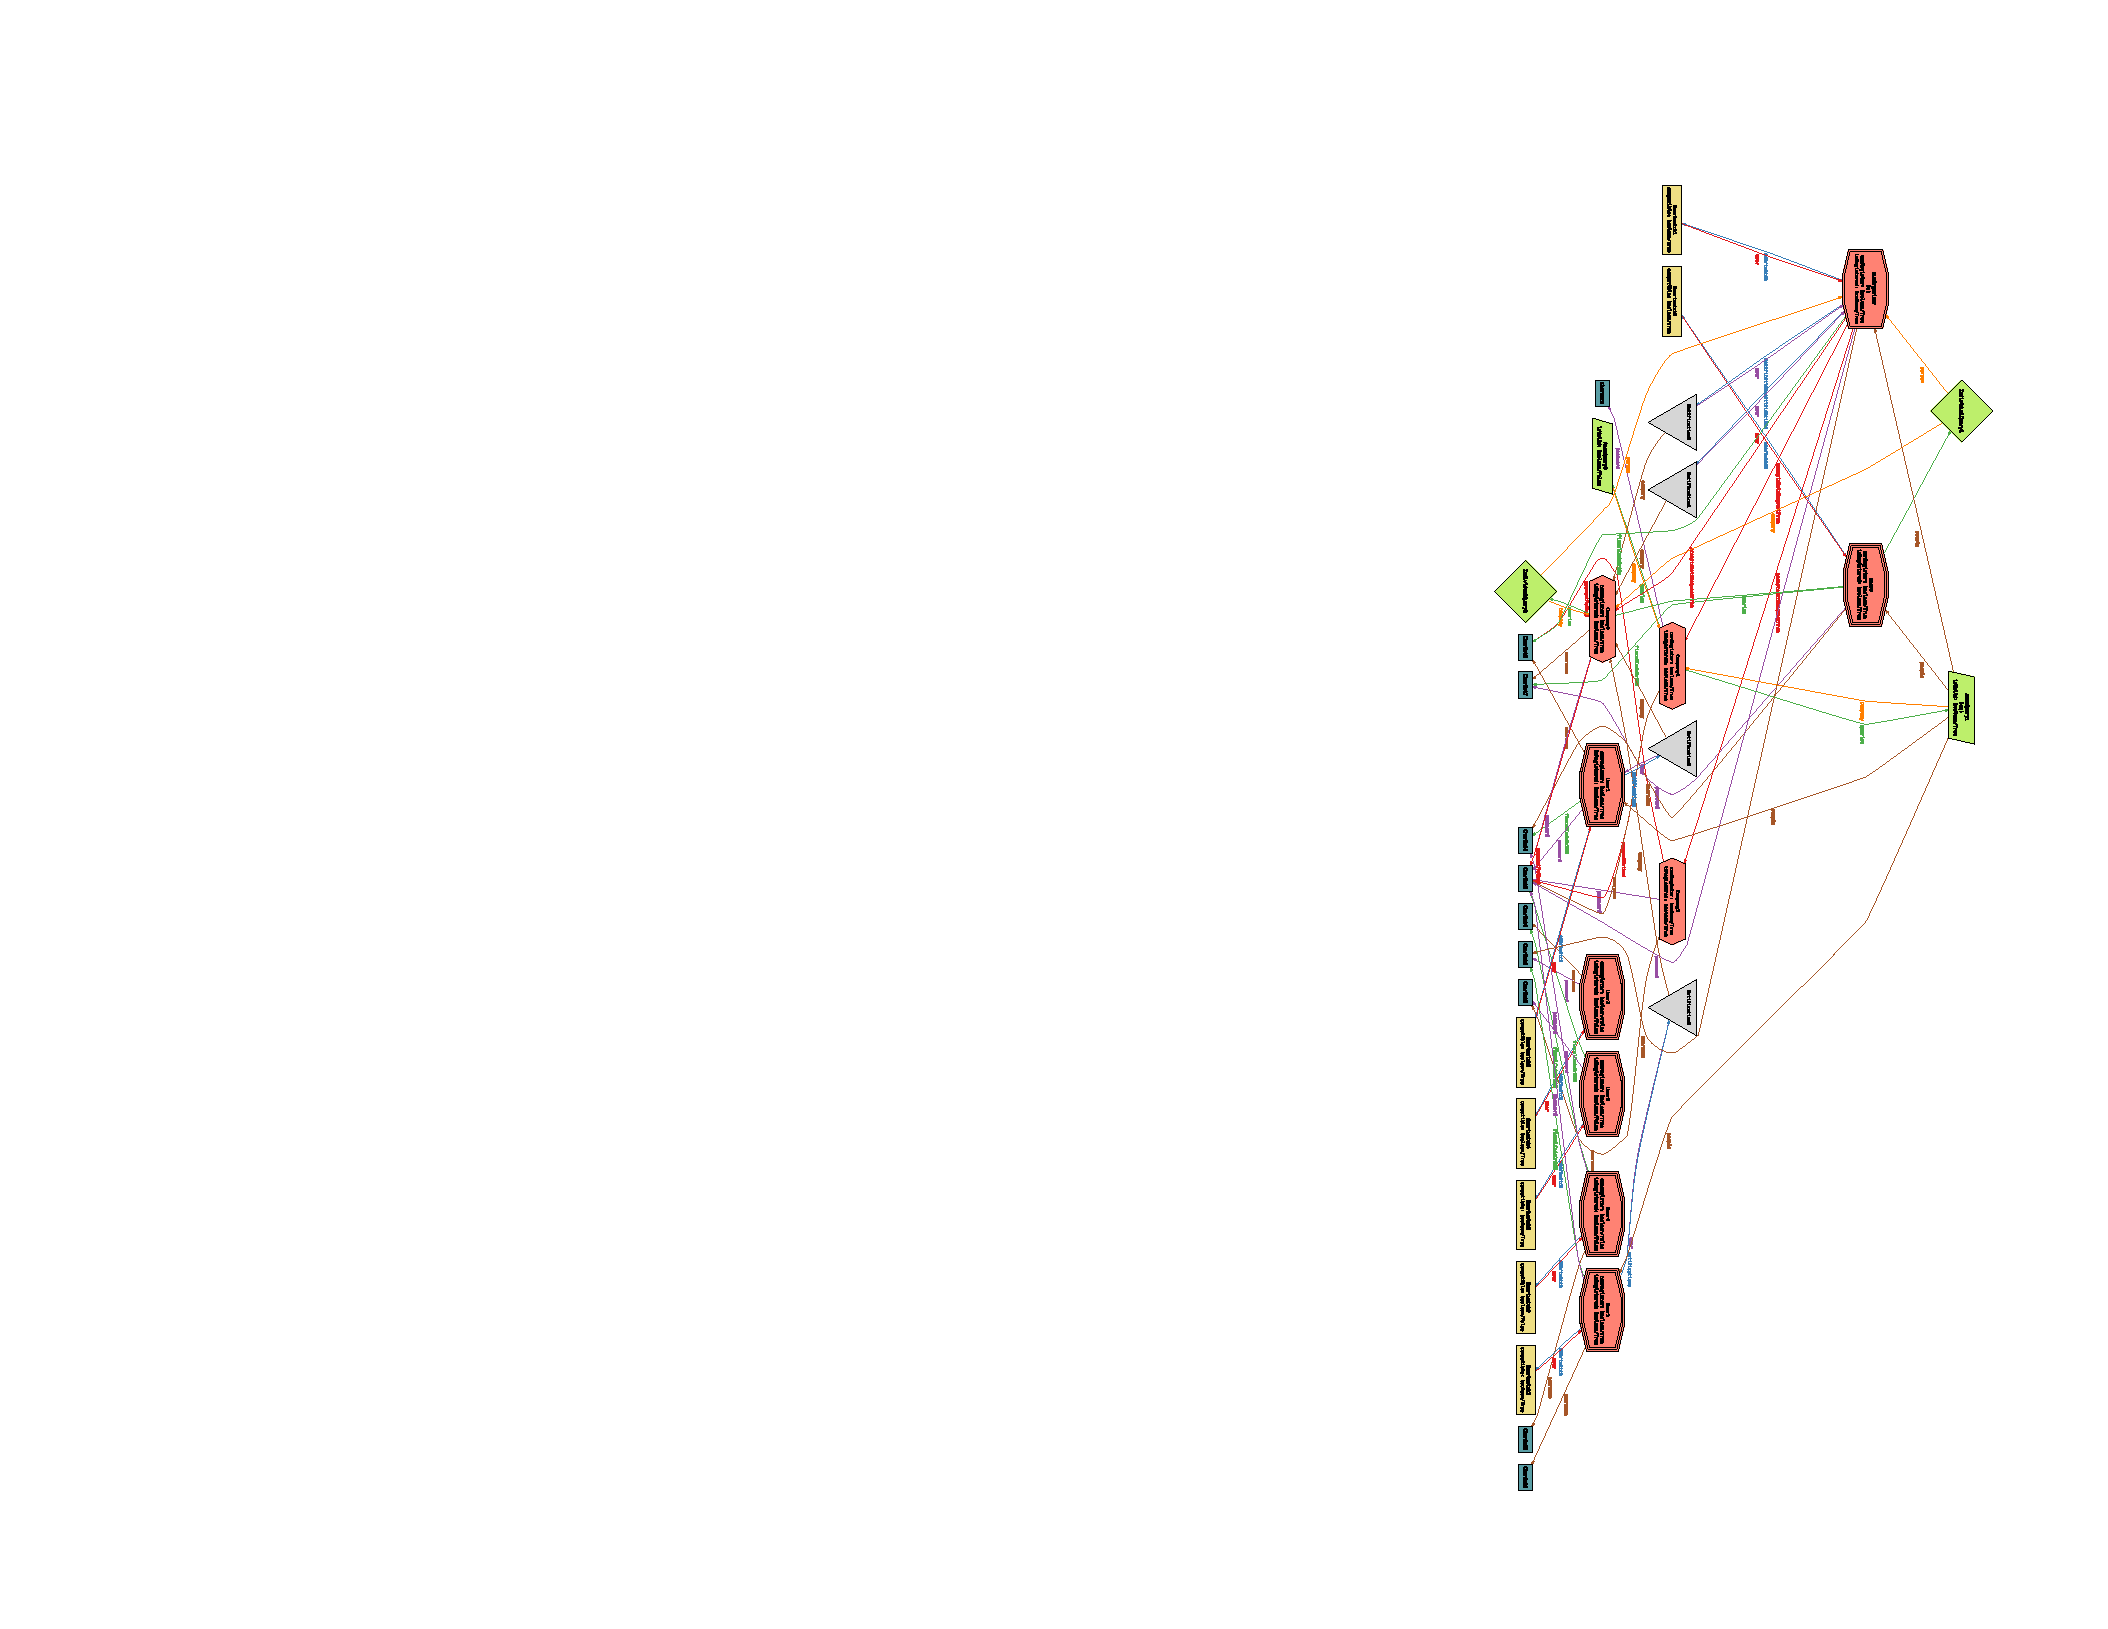
\includegraphics[height=18cm,width=10cm]{assets/worlds/cropped_showWithAnonQueryAllowed-rotated.pdf}
\end{center}
                \subsubsection{With Anonymous queries not allowed}
                \begin{center}
    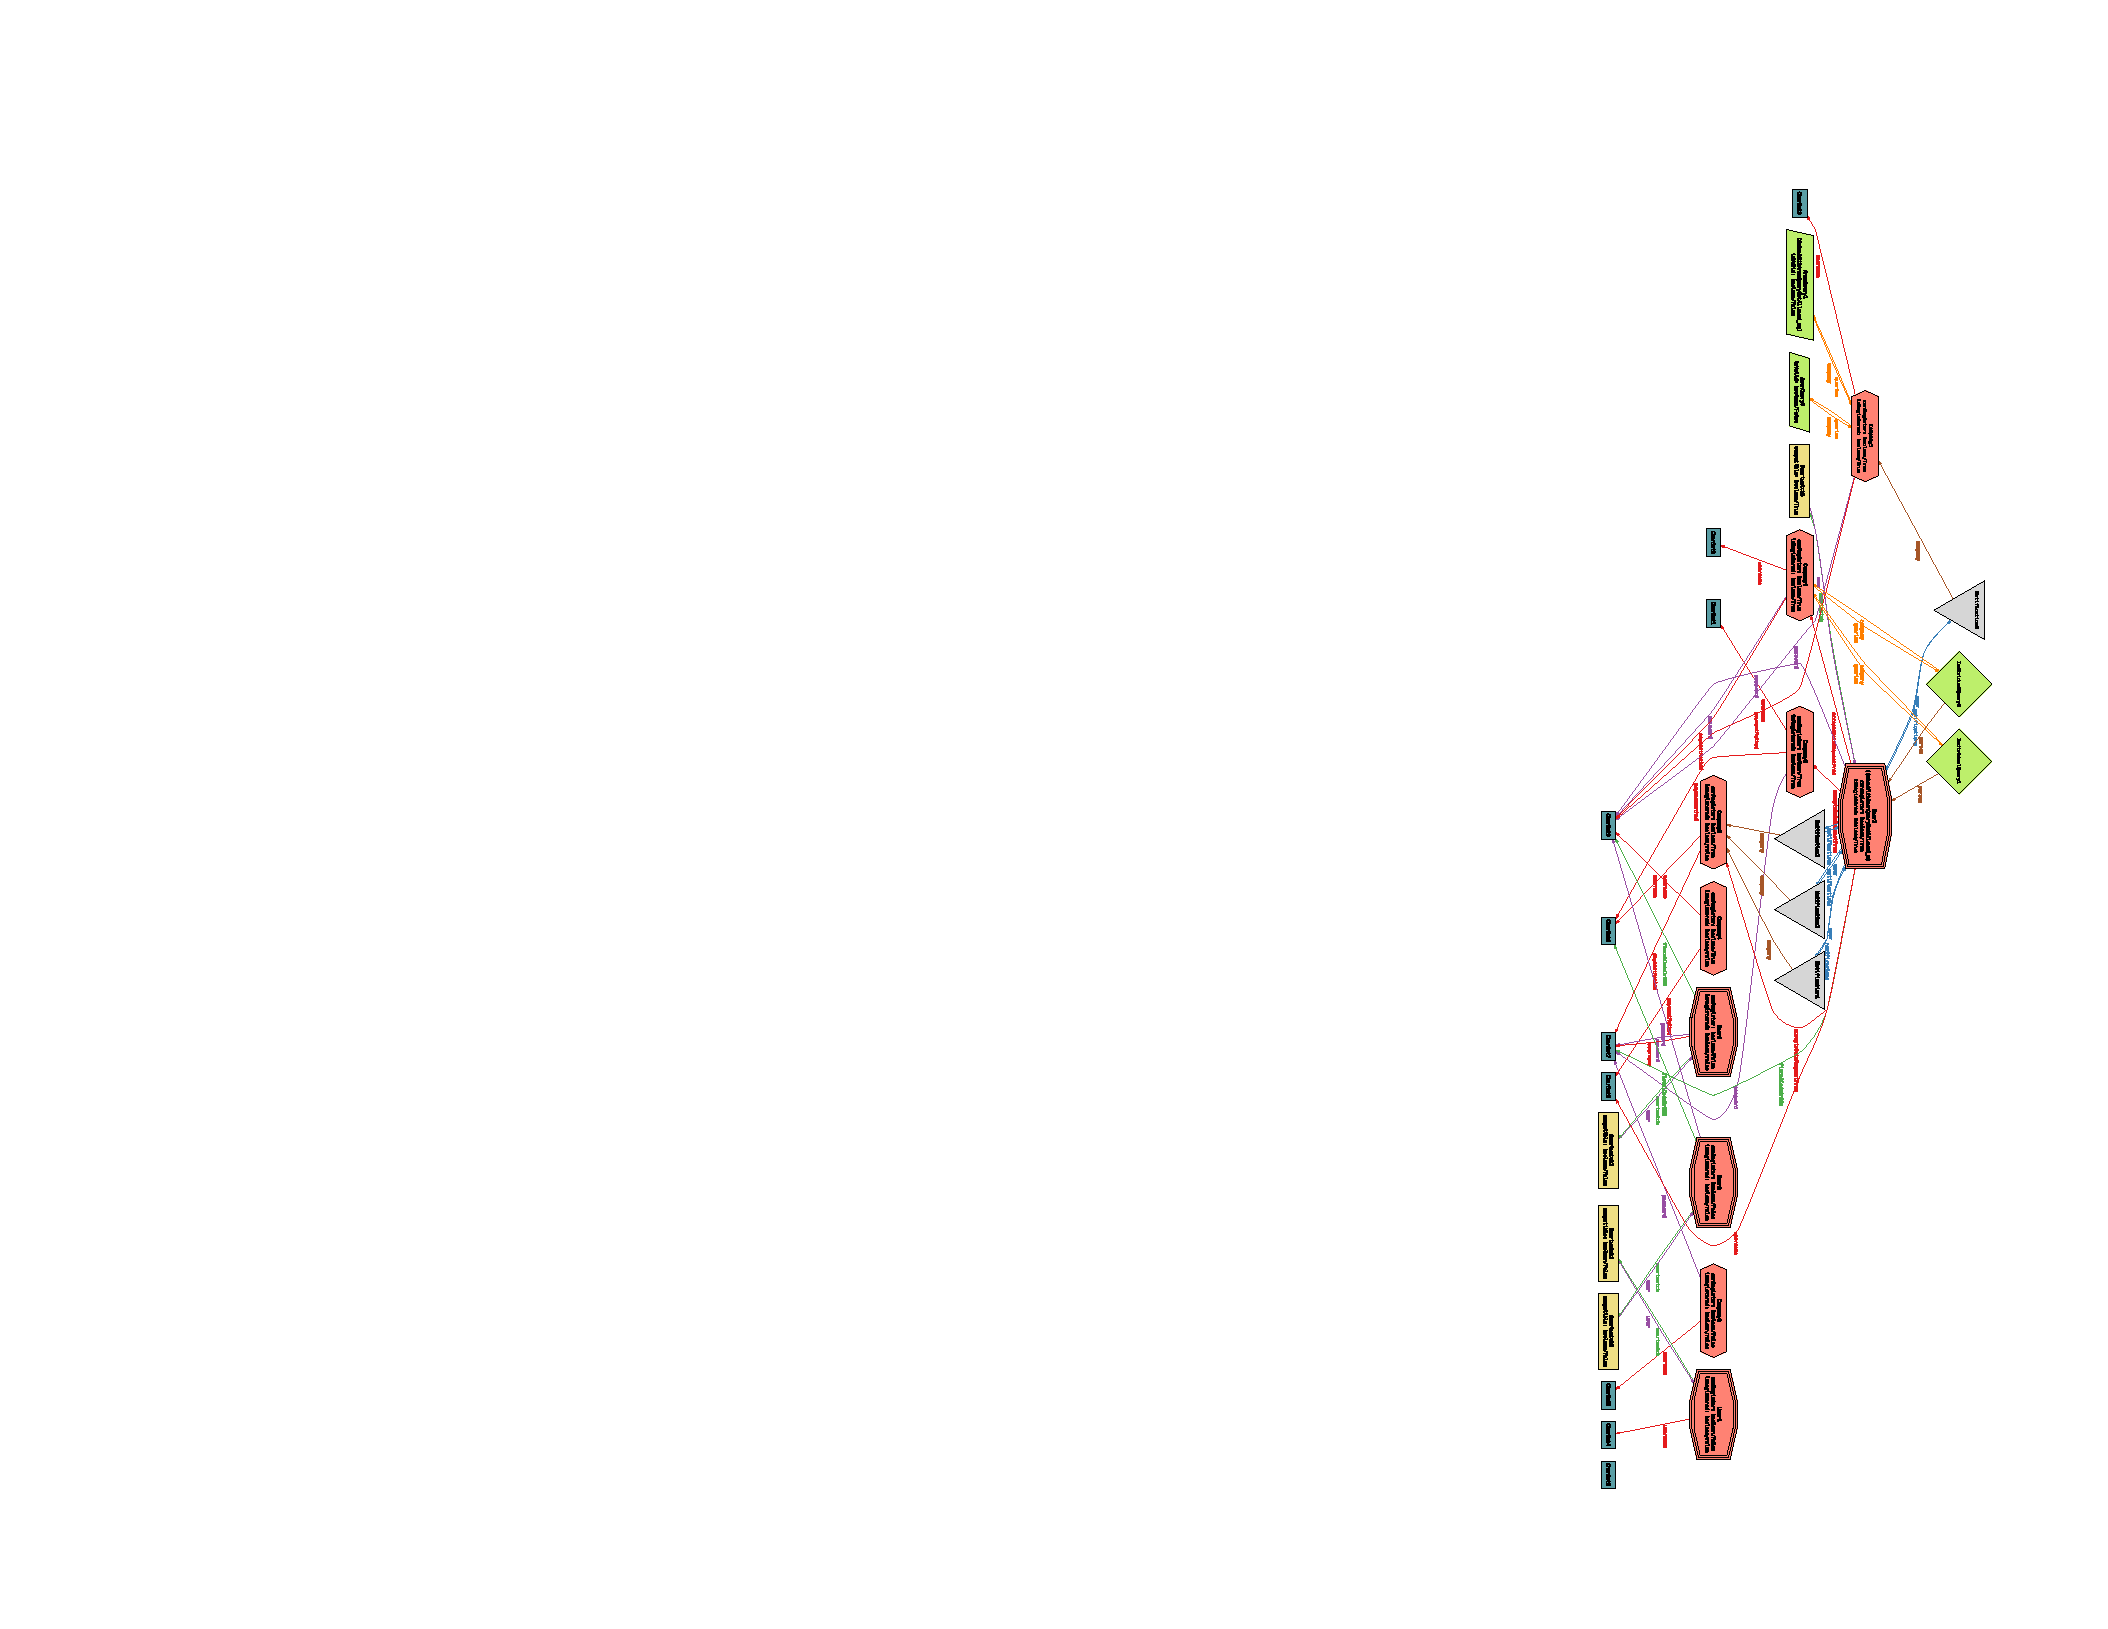
\includegraphics[height=18cm, width=10cm]{assets/worlds/cropped_showWithAnonQueryNotAllowed-rotated.pdf}
\end{center}
        \section{Hours tracking}
        \begin{tabular}{l*{6}{c}r}
            Date & Nicola Fossati & Daniele Montesi & Francesco Sgherzi \\
            \hline
            15/10/2018 & 2,5 & 2,5 & 2,5   \\
            \hline
            20/10/2018 & 0 & 4,0 & 4,0 \\
            \hline
            21/10/2018 & 1,5 & 1,5 & 2,5 \\
            \hline
            24/10/2018 & 0 & 2,5 & 0 \\
             \hline
            27/10/2018 & 3 & 2 & 0 \\
             \hline
            29/10/2018 & 5,5 & 5,5 & 5 \\
             \hline
            31/10/2018 & 0 & 4,5 & 0 \\
             \hline
            05/11/2018 & 4 & 0 & 4 \\
            \hline
            06/11/2018 & 5 & 1 & 6 \\
            \hline
            07/11/2018 & 10 & 2 & 9 \\
             \hline
            08/11/2018 & 4 & 0 & 2 \\
            \hline
            09/11/2018 & 3 & 0 & 4 \\
            \hline
            10/11/2018 & X & X & X \\


        \end{tabular}
\end{document}